\documentclass[twocolumn,preprintnumbers,amsmath,amssymb,superscriptaddress]{revtex4}
%\usepackage[pdftex]{graphicx}

\usepackage{amsmath,amsfonts,amssymb}
\usepackage[english]{babel}
\usepackage[latin1]{inputenc}
\usepackage[T1]{fontenc}
\usepackage{color}
\usepackage{float}
\usepackage{verbatim}
\usepackage{graphicx}
\usepackage{bm}
\usepackage{mathtools}
\usepackage{stmaryrd}
\usepackage{anyfontsize}

\usepackage[font={small}]{caption}
\usepackage{subcaption}
\captionsetup{compatibility=false}

%\usepackage{epstopdf}
%\usepackage{array}
%\usepackage{tabularx}
%\usepackage{multirow}
\usepackage{color}
%\usepackage{multibox}
%\usepackage{rotating}
%\usepackage{lineno}
%\usepackage[left]{lineno}
%\usepackage[comma,sort&compress]{natbib}
%\usepackage{authblk}
%\usepackage{multicol}

\usepackage{natbib}
\bibpunct{(}{)}{;}{a}{}{;}

\bibliographystyle{prsb}

\usepackage{bibunits}

\newcommand{\beginsupplement}{%
        \clearpage
        \setcounter{table}{0}
        \renewcommand{\thetable}{S\arabic{table}}%
        \setcounter{figure}{0}
        \renewcommand{\thefigure}{S\arabic{figure}}%
     }


%\linenumbers
%\setlength\linenumbersep{3pt}

\begin{document}


%\title{Simple rules yield complex communities: deconstructed species interactions and the assembly of communities}
%\title{Community assembly and dynamics by the deconstruction of species interactions}
\title{Eco-evolutionary dynamics and collective straying: implications for salmon metapopulation robustness}
\author{Justin D. Yeakel${}^{1,2,*}$, Jean P. Gibert${}^{1}$, Peter A. H. Westley${}^{3}$, \& Jonathan W. Moore${}^{4}$ \\
${}^1$School of Natural Sciences, University of California, Merced, Merced CA, USA \\
${}^2$The Santa Fe Institute, Santa Fe NM, USA \\
${}^3$College of Fisheries and Ocean Sciences, University of Alaska, Fairbanks, Fairbanks AK, USA \\
${}^4$Earth${}_2$Oceans Research Group, Simon Fraser University, Vancouver BC, Canada \\
${}^*$To whom correspondence should be addressed: jdyeakel@gmail.com
}




\begin{abstract} %250 words
The spatial dispersal of individuals is known to play an important role in the dynamics of populations, and is central to metapopulation theory.
At the same time, local adaptation to different environmental conditions creates a geographic mosaic of evolutionary forces, where the combined drivers of selection and gene flow interact.
Although the dispersal of individuals from donor to recipient populations provides connections within the metapopulation, potentially promoting demographic and evolutionary rescue, it may also introduce maladapted individuals into habitats that are host to different environmental conditions, potentially lowering the mean fitness of the recipient population.
Here we explore a minimal model of the eco-evolutionary dynamics between two populations connected by dispersal, where the productivity of each is defined by a trait complex that is subject to local selection.
Although general in nature, our model is inspired by salmon metapopulations, where dispersal between populations is defined in terms of the \emph{straying rate}, which has been shown to be density dependent, possibly emerging as a consequence of collective migration. 
The results of our model reveal that increased straying between evolving populations leads to alternative stable states, which has large and nonlinear effects on two measures of metapopulation robustness: the portfolio effect and the time to recovery following an induced disturbance.
We show that intermediate levels of straying result in large gains in robustness, and that increased differences between sites (increased habitat heterogeneity) promotes robustness when straying rates are low, and erodes robustness when straying rates are high.
Finally, we show that density-dependent straying promotes robustness, particularly when the aggregate biomass is low and straying is correspondingly high, and this has important ramifications for the conservation of salmon metapopulations facing both natural and anthropogenic disturbances.
\end{abstract} %250 words


\maketitle

Intraspecific diversity can increase the resilience and stability of species or metapopulations. 
This diversity-stability linkage can occur when there are asynchronous population dynamics, where the changes in population size varies across the metapopulation. 
This asynchrony will increase the potential for demographic rescue \cite{Brown:1977gk,Earn:2000fm} and also decrease the variability of processes that integrate across the metapopulation \cite{Anonymous:2015gf}. 
For example, different responses to climate variability within populations of a rare plant reduced fluctuations in abundance \cite{Abbott:2017hl}. 
This statistical buffer has traditionally been quantified as the Portfolio Effect (PE), which is the ratio of the population CV to the CV of the aggregated metapopulation \cite{Thibaut:2012km}. 
Strengthened portfolio effects are expected to increase the robustness of metapopulations to external disturbances, and by extension promote persistence \cite{Thibaut:2012km}.
In contrast, homogenization of populations leading to greater synchronization and weakened PE may be a harbinger of metapopulation collapse and extinction.


% Although dispersal and the consequent gene flow can influence the evolutionary dynamics of metapopulations, the interplay between selection, population dynamics, and persistence is not well understood.
Movement of individuals among local populations (i.e. dispersal) can have a large influence on metapopulation persistence \cite{MilnerGulland:2011vm}. 
Dispersal facilitates evolutionary rescue, whereby immigration of individuals with heritable adapative traits can rescue small populations from local extinction in the context of maladaptive environmental change \cite{Bell:2011ki,Carlson:2014is}.
% First, some level of straying is necessary to enable the rescue effect, whereby dispersal among populations can rescue small populations from local extinction (REFS). 
On the other hand, high rates of dispersal may synchronize populations and actually increase the risk of extinction of the entire metapopulation \cite{Earn:2000fm}. 
Third, straying will influence the evolutionary dynamics of the metapopulation.
% though how the interplay between selection and population dynamics might impact persistence is less well understood. 
Although the dispersal of individuals into sites hosting other populations provides connections within the larger metapopulation, potentially promoting demographic and evolutionary rescue, it may also introduce maladapted individuals into habitats that are host to different environmental conditions, possibly lowering the mean fitness of the recipient population \cite{Muhlfeld:2014hs}. 
More broadly, dispersal can provide a mechanism by which phenotypes are sorted in space rather than time and facilitates the spread of maladaptive genes \cite{Lowe:2015ft}.
Further, this straying may lead to genetic homogenization that erodes the asynchrony that underpins portfolio effects and metapopulation persistence. 
Thus, straying can influence the resilience and robustness of metapopulations through both ecological and evolutionary processes.
% Thus, the dual nature of straying as both promoter of connections among metapopulation demes and potential eroder of locally adapted gene complexes highlights the interplay between ecological dynamics of connected populations and the evolutionary dynamics of mixed trait distributions that respond to heterogeneous local conditions.


%Movement through space (link back to straying)
% Migratory populations that return to a breeding ground or natal stream to reproduce are linked to each other by some proportion of the population that permanently disperse, or stray into the `wrong' site. %; we might say that there is at least one \emph{Kevin} in every school or flock (figure \ref{fig:xkcd}).
There is growing appreciation that a combination of abiotic, biotic, and anthropogenic factors can control the rate of dispersal among populations \cite{H:2013fs,Keefer:2014gg,Bett:2017ha}.
Migratory populations that return to breeding sites for reproduction are linked to each other by some proportion of the population that permanently disperses into the `wrong' site. 
Recently, the role of social interactions and collective navigation has been hypothesized [This issue].
The rate at which individuals stray, $m$, may be linked to errors made at an individual-level that are themselves diminished by migrating in groups and pooling individual choices \cite{Simons:2004jo,Berdahl:2015kv,Berdahl:2016dx}.
The potential influence of collective dispersal on the dynamics of individual populations and the metapopulation as a whole is a topic of considerable interest that has tangible conservation implications \cite{Brenner:2012gl,Johnson:2012fe,Fullerton:2011ii}.
% Whether and to what extent the ecological consequences of straying depend on the evolutionary dynamics that emerge from populations distributed across a selective gradient is unclear.
% How the assumed negative evolutionary effects of straying and subsequent gene flow is balanced by the positive effects of demographic rescue is the subject of this contribution.



%Eco-evolutionary dynamics in space
%% From geographic mosaic of coevolution to...
% That evolutionary forces of selection and gene flow play out heterogeneously across geographic mosaics is now a foundational concept in ecology and evolutionary biology \cite{Nuismer:1999ko,Thompson:2015hq,Nuismer:2000bb,Thompson:2005wf}.
% These mosaics are in part driven by environmental differences between habitats that alter the selective forces acting on different phenotypes \cite{Endler:1986tz}, and a principle underlying assumption is that there is gene flow such that individuals from different habitats mix over space \cite{Gomulkiewicz:2000bz,Thompson:2002hr,Nuismer:2003eh,Nuismer:2006be,Forde:2008kc,Guimaraes:2011hu,Gibert:2013hp}.
% Although the evolutionary outcomes of these spatial processes have been explored in depth (REFS), it is less well understood how selective mosaics and their consequent evolutionary forces impact population dynamics as they unfold \cite{Hendry:2016un}.


%Motivation: straying
The eco-evolutionary impacts of dispersal likely has important implications for conservation and management in key taxa such as in migratory salmon.
While anadromous salmonid fishes (genera \emph{Oncorhynchus} and \emph{Salmo}) are renown for returning to their natal spawning habitats with high accuracy and precision after years at sea \cite{Quinn:2011tf,Jonsson:2011kg,Keefer:2014gg}, there are generally some individuals that `stray' to non-natal sites to spawn \cite{Quinn:1993ge,Hendry:2004wf}.
Salmon may operate as metapopulations, where populations are genetically distinct but linked by some level of straying \cite{Schtickzelle:2007wb,Anderson:2014cx}.
Although extensive work has been done to document the extent of straying from donor populations and into recipient populations \cite{Keefer:2014gg,Bett:2017ha}, only recently have the abiotic, biotic, and anthropogenic influences of `straying' behaviors been investigated systemically \cite{Keefer:2008bs,Westley:2015to,Bond:2016dz}.
Straying among salmon may be influenced by environmental factors such as water temperature, human activities such as hatchery practices, and population density as predicted by the collective migration hypothesis \cite{Peterson:2014gy}.
These strays can introduce new maladaptive genotypes into the recipient population.
Further, straying and genetic homogenization could synchronize population dynamics and erode portfolio effects \cite{Moore:2010gs,Carlson:2011ce,Braun:2016ib}.
Thus, there is opportunity and a need to consider the eco-evolutionary consequences of straying for metapopulations in species of conservation and management concern such as salmon. 

% Asynchrony among salmon populations also increases the stability of fisheries that integrate across this diversity \cite{Schindler:2010he,Anonymous:2016jc}.
% However, these portfolio effects may be eroded if asynchrony is influenced by genetic diversity and this genetic diversity is lost. 
% Braun et al. \cite{Braun:2016ib} found that genetic differences among populations of Chinook salmon was correlated with the degree of asynchrony in population dynamics. 
% Artificial propagation of salmon by hatcheries and their strays may erode local genetic diversity, asynchrony among populations, and portfolio effects \cite{Carlson:2008hl,Moore:2010gs,Anonymous:2014ku}.  
%Coordinated mass migrations are one of the great wonders of the natural world, and the ability of individuals and groups to navigate across great distances have long fascinated naturalists \cite{MilnerGulland:2011vm}.

% Most recently the role of social interactions and collective navigation has been hypothesized \cite{Berdahl:2015kv,Berdahl:2016dx}.
% These strays can introduce new maladaptive genotypes into the recipient population.
% Straying amon salmon may be influenced by environmental factors such as water temperature, human activities such as hatchery practices, and population density as predicted by the collective migration hypothesis \cite{Peterson:2014gy}. 
% Thus, there is an opportunity to consider the eco-evolutionary consequences of straying for metapopulations in species of conservation and management concern such as salmon \cite{Carlson:2011ce}. 

% 
% \begin{figure}
%   \captionsetup{justification=raggedright,
% singlelinecheck=false
% }
% \centering
% 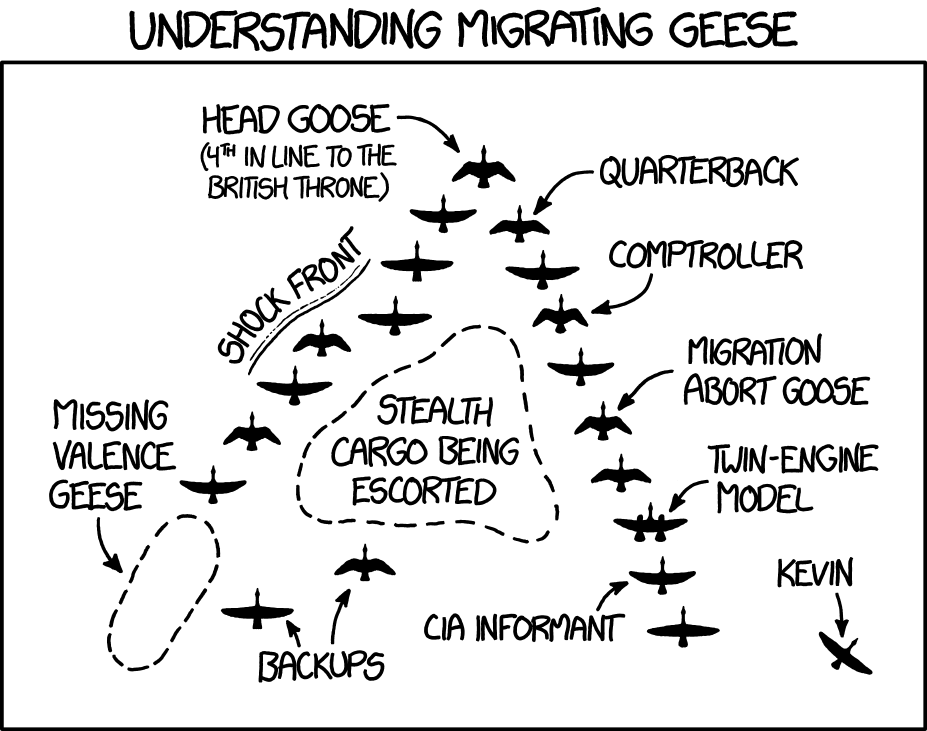
\includegraphics[width=0.4\textwidth]{figs2/fig_xkcd.png}
% \caption{
% \emph{Migrating Geese}, a comic from Randall Monroe's xkcd (https://xkcd.com/1729/). 
% A flock of geese travel in the direction of a shared destination, the lone stray named \emph{Kevin}.
% In this case, the rate of straying is $m=0.05$, which is not an uncommon rate for migrating populations of salmon \cite{Satterthwaite:2015ge}. 
% Reprinted under the Creative Commons Attribution-NonCommercial 2.5 License.
% } \label{fig:xkcd}
% \end{figure}

%Alternative stable state
Here we seek to explore how collective density-dependent straying influences the stability and robustness of metapopulations through ecological and evolutionary processes.
% the potentially detrimental evolutionary effects of straying (erosion of local adaptation) and subsequent gene flow is balanced by the positive effects of demographic rescue is the subject of this contribution.
% Here we ask the overarching question: how does collective behavior mediated dispersal and gene flow interact to influence the robustness of locally adapted populations?
To address this question we construct a minimal eco-evolutionary model of two populations occupying different sites that are linked by straying individuals, each of which with an associated trait distribution subject to natural selection determined by local conditions.
Specifically we compare (a) different rates of straying and (b) the influence of collective movement, across (c) increasing environmental heterogeneity, by assessing two measures of metapopulation robustness: the portfolio effect and the time required for a population(s) to recover following an induced disturbance. 
This model enables us to explore the multiple and potentially opposing pathways by which straying influences metapopulation robustness such as the potentially detrimental erosion of local adaptation vs. the positive effects of demographic and evolutionary rescue.
% [We show that taking straying into account leads to alternative stable states in population densities and trait values, which has consequences for maladaptation, intraspecific trait variability, and long-term sustainability of salmon metapopulations.]



\section{Model Description \& Analysis}

\noindent{\bf (a) Metapopulation framework}\\
\noindent We consider two populations $N_1$ and $N_2$ that inhabit two distinct habitats, each with trait values $x_1$ and $x_2$ determing recruitment rates.
We assume that there is an optimum trait value $\theta_1$ and $\theta_2$ associated with each habitat, where recruitment is maximized if the trait value of the local population equals the optimum, such that $x = \theta$.
Moreover, we assume that $x_{1,2}$ are normally distributed with means $\mu_1$ and $\mu_2$ and have the same standard deviation $\sigma$.
As such, the recruitment rate for both populations is determined by the mean trait value of the local population, such that $r_1 = R_1[\mu_1(t),\theta_1]$.
Trait means for each population are subject to selection, the strength of which depends on the difference between the trait mean and the local trait optimum at a given point in time \cite{simpson1953major,Lande:1976ga}.

%PW: Can we say anything about the effect of the recipient population size and that effect on evolutionary dynamics? Again, straying can be thought of as both from the donor or recipient population perspective.
The two populations occur in spatially separate sites that are close enough such that a proportion of the population $m$ can stray into the other site, and where mortality occurs before individuals return to reproduce.
If there is no straying between these populations, then the mean trait evolves towards the optimal value for each site $x_1 \rightarrow \theta_1$, and the recruitment rate for each population is maximized.
If there is straying between populations at rate $m$, then the traits in each respective location will be pulled away from the optimum, and recruitment rates will be lowered.
As $m \rightarrow 0.5$, the populations are perfectly mixed, acting as a single population.

\begin{figure}
  \captionsetup{justification=raggedright,
singlelinecheck=false
}
\centering
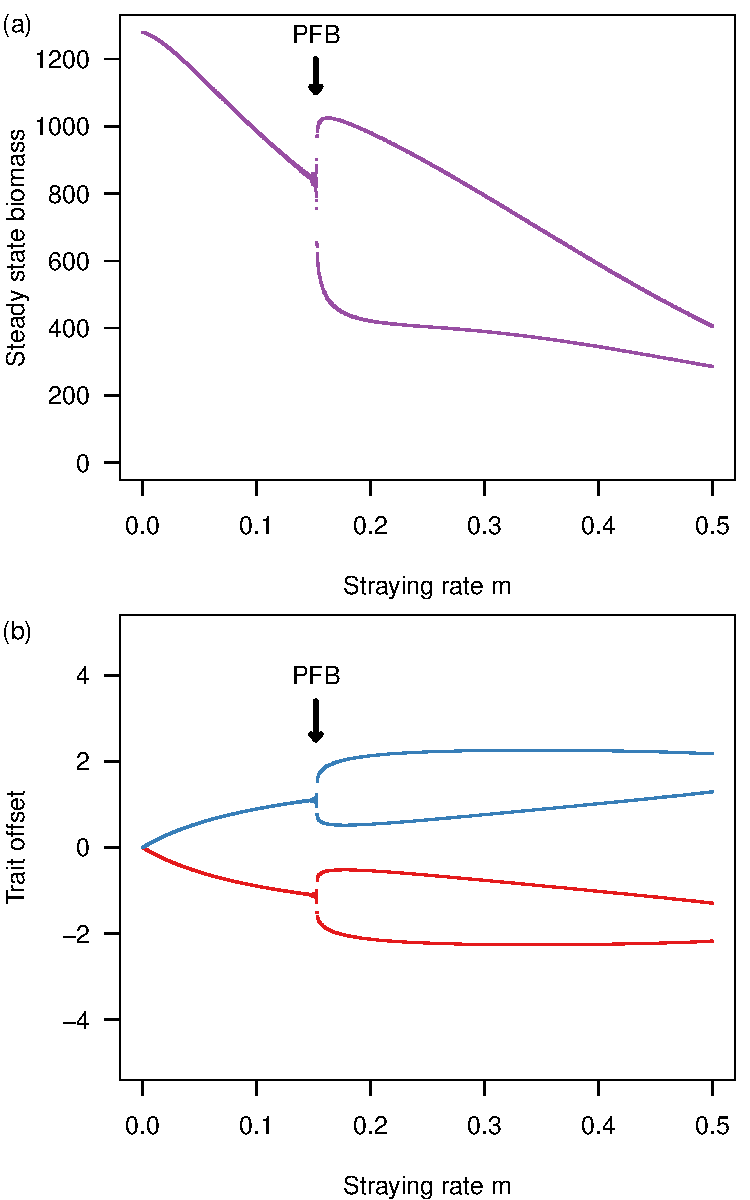
\includegraphics[width=0.4\textwidth]{figs2/fig_traj.pdf}
\caption{
A) The steady state densities of $N_1$ and $N_2$ as a function of a constant stray rate $m$. Which population attains the low- or high-density state is random due to small applied fluctuations in the initial conditions.
B) The steady state trait values measured as $\theta_i - x_i$, as a function of a constant stray rate $m$. 
FB marks the fold bifurcation.
} \label{fig:traj}
\end{figure}

We use discrete Ricker framework described by Shelton and Mangel \cite{Shelton:2011eq} as the basis for our two-site metapopulation model, with the added effect of the local population $N_i$ mixing with a set proportion $m$ of a remote population $N_j$ that is straying into it.
In this sense, both populations serve simultaneously as donor and recipient populations.
We first assume that the proportion ${\rm e}^{-Z}$ of both populations survive such that the surviving aggregated population, composed of both local individuals (at site $i$) and incoming strays (from site $j$), is $\left((1-m)N_i(t) + m N_j(t) \right){\rm e}^{-Z}$.
Because local individuals will recruit differently than incoming strays, the recruitment of the aggregate must incorporate two recruitment functions, given by $\left(R_i[\mu_i(t)] (1-m)N_i(t) + R_i[\mu_j(t)] m N_j(t)\right)$.
This mix of individuals is subject to the same compensatory effects, which is determined by the parameter $\beta$.
Taken together, the difference equation that determine changes in population size is

\begin{align}
  &N_i(t+1) = \\ \nonumber
  &\left((1-m)N_i(t) + m N_j(t) \right){\rm e}^{-Z} \\ \nonumber
  &+ \left(R_i[\mu_i(t)] (1-m)N_i(t) + R_i[\mu_j(t)] m N_j(t)\right) \\ \nonumber
  &\times {\rm e}^{-\beta ((1-m)N_i(t) + m N_j(t))},
  \label{eq:N}
\end{align}

\noindent where the difference equation for $N_j$ mirrors that for $N_i$.

The recruitment of local individuals $(1-m)N_i(t)$ as a function of their mean trait value at time $t$ and the local trait optimum, is

\begin{align}
  &R_i[\mu_i(t)] = \\ \nonumber
  &\int_{-\infty}^\infty r_{\rm max}\exp\left\{\frac{(x_i(t)-\theta_i)^2}{2\tau^2}\right\} {\rm pr}(x_i(t),\mu_i,\sigma^2) {\rm d}x_i(t) +\tilde{P}\\ \nonumber
  &= \frac{r_{\rm max} \tau  }{\sqrt{\sigma ^2+\tau ^2}}\exp\left\{-\frac{(\theta_i-\mu_i(t))^2}{2 \left(\sigma ^2+\tau ^2\right)}\right\} +\tilde{P},
  \label{eq:R}
\end{align}

\noindent where the mismatch between the local trait mean $\mu_i(t)$ and the local optimum $\theta_i$ scales the recruitment rate for the population, and $\tilde{P}\sim {\rm Normal}(0,0.01)$ introduces a small amount of demographic error.
The parameter $\tau$ is the strength of selection, and controls the sensitivity of recruitment to changes in the mean trait value away from the optimum (the strength of selection increases with smaller values of $\tau$), which we set as $\tau=1$ here and throughout.
Because straying individuals are emigrating from a population with a mean trait value farther from the local optimum, their rate of recruitment is diminished.
Recent studies of wild sockeye salmon have indeed found that straying individuals have lower life-time fitness than individuals that do not stray, although it unknown at what life-stage this selection occurs \cite{Peterson:2014gy}.
% The compensatory effects are then determined by the exponential, following the Ricker stock-recruitment relationship.
\\

\begin{figure*}
  \captionsetup{justification=raggedright,
singlelinecheck=false
}
\centering
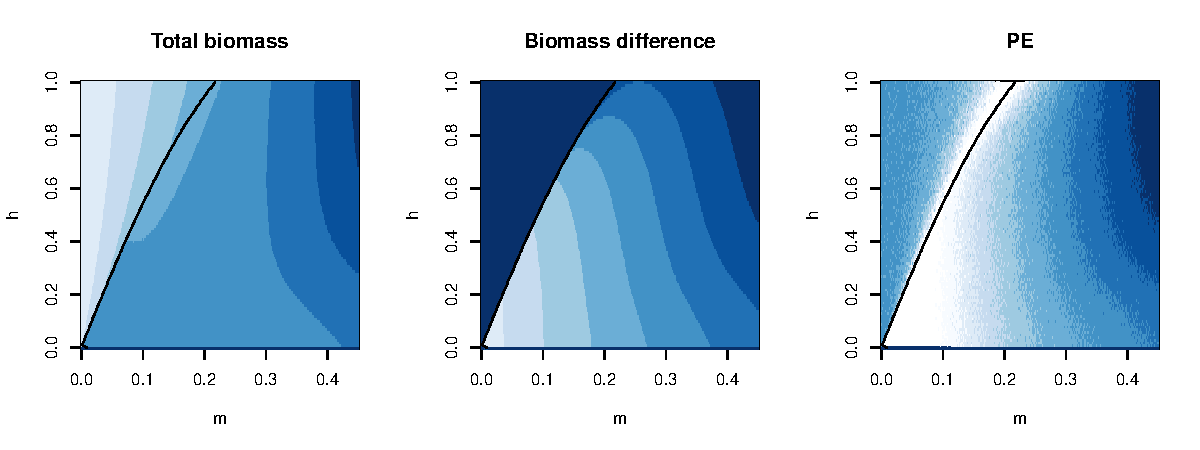
\includegraphics[width=0.8\textwidth]{figs2/fig_MDPE_hm.pdf}
\caption{
(a) Total means $N_t$, (b) difference in means $\Delta N$, and (c) the portfolio effect PE as a function of heritability $h^2$ and a constant stray rate $m$. Light colors = high values.
The black line shows the fold bifurcation separating a single steady state (left) from alternative stable states (right).
(d) The relationship between the time to recovery following a disturbance and the portfolio effect.
The black line denotes the fold bifurcation.
} \label{fig:PE}
\end{figure*}

% \noindent{\bf (b) Recruitment over a selective landscape}
\noindent Because individuals from the local population are mixed with individuals from the remote population via straying and subsequent reproduction, the resulting trait distribution is a mixed normal with weights corresponding to the proportion of the mixed population that are local individuals, $w_i$, and for the straying individuals, $1-w_i$, where 
\begin{equation}
w_i=\frac{(1-m)N_i(t)}{(1-m) N_i(t) + m N_j(t)}.
\end{equation}
We make two simplifying assumptions.
First, we assume that the distribution resulting from the mix of remote and local individuals, following reproduction, is also normal with a mean value equal to that of the mean for the mixed-normal distribution.
Thus, we assume that strays can successfully reproduce and introduce their genotypes into the recipient population, which is supported by observations in wild populations \cite{Jasper:2013cc}.
Second, we assume that changes in trait variance through time are minimal, such that $\sigma^2$ is assumed to be constant, which is a common simplification in eco-evolutionary models of population dynamics \cite{Lande:1976ga,Schreiber:2011wx,Gilbert:2014ee,Gibert:2015kc}.



% An increasing flow of incoming strays is generally expected to pull the mean trait value of the local population away from its optimum over time, which will decrease its rate of recruitment.
Following Lande \cite{Lande:1976ga}, the mean trait value thus changes through time according to the difference equation

\begin{align}
  \label{eq:mu}
  \mu_i(t+1) &= w_i\mu_i(t) + (1-w_i)\mu_j(t) \\ \nonumber
  &+ h^2\sigma^2\frac{\partial}{\partial \mu_i}\ln\left(w_i R_i[\mu_i(t)] + (1-w_i)R_i[\mu_j(t)]  \right),
\end{align}

\noindent where the first two components determine the mixed normal average of the aggregated local and remote populations.
The partial derivative in the Eq. \ref{eq:mu} determines how the mean trait changes through time due to natural selection \cite{Lande:1976ga}, which is proportional to the change in mean fitness with respect to $\mu_i$.
\\



\noindent {\bf (b) Density-dependent straying}
%Density dependent m
\noindent We have so far assumed that the proportion of strays leaving and entering a population is constant, however there is mounting evidence that at least in some species (including salmon) the straying rate is density-dependent with a signature of collective navigation \cite{Berdahl:2016dx,Bett:2017ha}.
Specifically, the rate at which individuals stray has been linked directly to a collective decision-making phenomenon, where greater numbers of individuals tend to decrease the rate at which individuals err, reducing the overall proportion of a population that strays.
According to Berdahl et al. \cite{Berdahl:2014bl,Berdahl:2016dx}, given the probability that an individual strays is $m_0$, the proportion of the local population $N_i(t)$ that strays is

\begin{equation}
  m(t) = m_0\left(1- \frac{N_i(t)}{C+N_i(t)}\right),
  \label{eq:ddm}
\end{equation}

\noindent where $C$ is a half-saturation constant.
We note that at the limit $C\rightarrow \infty$, the density-dependent straying rate becomes constant such that $m(t) \rightarrow m_0$, and this corresponds to the original formulation where $m=m_0$.
A similar observation shows that when the population density is very high, $m(t) \rightarrow 0$, and when it is small, individuals operate without regard to collective behavior, meaning $m(t) \rightarrow m_0$.
Thus, for realistic population densities, $m(t) < m_0$.\\


\noindent {\bf (c) Habitat heterogeneity}
\noindent Increasing differences in optimal trait values between sites ($\Delta\theta = \left|\theta_i - \theta_j\right|$) corresponds to greater regional differences in the conditions that favor alternative trait complexes, which we interpret here as increased habitat heterogeneity.
If both populations are isolated, natural selection will direct the mean trait values of both populations towards their respective optima, such that $\mu_i(t) \rightarrow \theta_i$ as $t\rightarrow\infty$.
%difference in optimal trait values between the local and remote populations, which we call . 
%Linking m/m0 and thetadiff
Although we largely treat habitat heterogeneity and the rate of straying as independent parameters, we evaluate a case where we assume thgat increased habitat heterogeneity correlates with lower straying rates, and vice versa.
Two scenarios may lead to this correlation: 
(\emph{i}) sites may be distributed over greater spatial distances, where habitat dissimilarity is assumed to be larger between more distant sites, whereas the likelihood of straying over greater distances would likewise be lower \cite{Candy:2000hu,JPE:JPE1383};
(\emph{ii}) individuals may have behaviors promoting dispersal between habitats with structural or physiognomic similarities \cite{Peterson:2014gy}.

Where indicated, we account for correlation between the straying rate and the differnce between optimal trait values by assuming that $m$ (if the stray rate is constant) or $m_0$ (if the stray rate is density-dependent) is a function of the difference between optimal trait values between sites $\Delta\theta$.
The straying rate is maximized at $m_{\rm max} = 0.5$, assuming both sites are equally attractive to the respective populations.
Thus, we can integrate these two variables by setting $m,m_0 = (1/m_{\rm max} + \epsilon \Delta\theta)^{-1}$, where $\epsilon$ sets the sensitivity of a declining $m$ to increasing distance (greater values of $\Delta\theta$), which we set to $\epsilon=2$.\\


\noindent {\bf (d) Measuring metapopulation robustness}
\noindent We evaluated metapopulation robustness by measuring the average-CV portfolio effect (PE) \cite{Anderson:2014cx,Schindler:2015gf} as well as the time required for the system to return to a steady state following an induced disturbance to one or both of the populations \cite{Ovaskainen:2002il}.
The average-CV portfolio effect is, as the name implies, the average CV across each population divided by the CV of the aggregate \cite{Anderson:2013gb}, such that


\begin{equation}
\langle{\rm PE}\rangle =\frac{1}{X}\sum_{i=1}^{X} \frac{\sqrt{{\rm VAR}(N_i)}}{{\rm E}(N_i)}\cdot \frac{{\rm E}(N_T)}{\sqrt{{\rm VAR}(N_T)}},
\label{eq:pe}
\end{equation}

\noindent where in this case the number of populations is limited to $X=2$ and the expectations $\rm E(\cdot)$ and variances $\rm VAR(\cdot)$ are evaluated at the steady state.
As the CV of $N_T$ decreases relative to that of the constituent populations, $\langle{\rm PE}\rangle > 1$, and the metapopulation is presumed to become more stable.
Portfolio effects greater than unity corresponds to less synchronization  \cite{Loreau:2008ju,Anderson:2014cx,Yeakel:2013vz} and thus a greater potential for demographic rescue among populations, buffering the system as a whole against extinction. 

%Although there are more robust ways to measure the portfolio effect (in particular for comparing the PE across species with different mean-variance relationships; REF: Anderson), its only utlity here is to provide a simple statistical measure of metapopulation persistence.
A more direct way to measure system robustness is to measure the time that the system (measured as the aggregate biomass $N_T$) takes to recover its steady state abundance following an induced disturbance: systems that recover quickly (shorter recovery times) are more robust than those that recover more slowly (longer recovery times).
Although there is a direct eigenvalue relationship between the rate of return following a small pulse perturbation \cite{GuckHolmes}, because we aimed to 1) assess the effects of a large perturbation, and 2) estimate the time required for all transient effects to decay (including dampened oscillations), we used a simulation-based numerical procedure.

Numerically estimating the time that it takes for a perturbed system to relax also permits a more detailed perspective of metapopulation fragility.
For example, if populations settle to alternative stable states (alternative stable states in our model requiring one population to be high-density and one low-density), comparing recovery times after a disturbance applied to the high, low, and/or both populations allows for an assessment of which component of the metapopulation has a longer-lasting influence on the system's recovery.
We measured recovery time following three types of induced disturbance: (\emph{i}) extinction of the low-density population; (\emph{ii}) extinction of the high-density population (scenarios \emph{i} and \emph{ii} are equivalent if the system is in the single steady state regime); (\emph{iii}) near-collapse of both populations where just 1.0\% of each survives.
Throughout, we will refer to an increase in the portfolio effects and/or reduction in recovery times as promoting metapopulation robustness, which is expected to have a positive effect on persistence.
\\


\section{Results}


\begin{figure}
  \captionsetup{justification=raggedright,
singlelinecheck=false
}
\centering
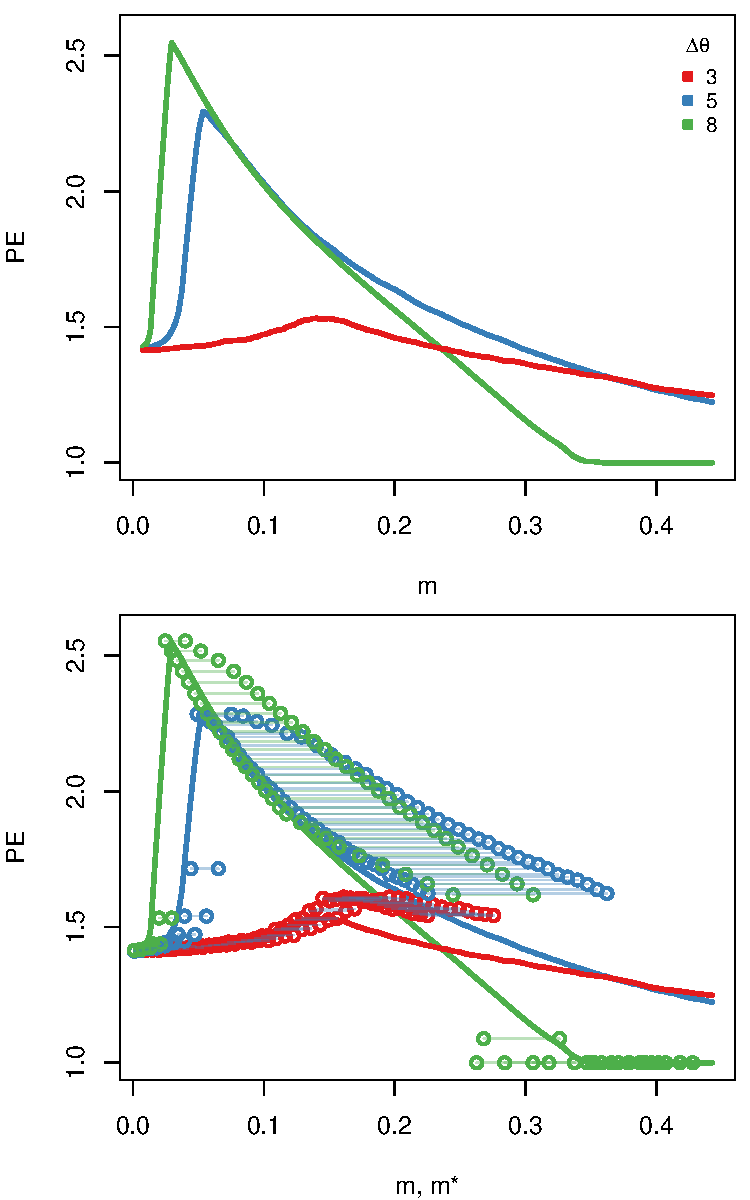
\includegraphics[width=0.4\textwidth]{figs2/fig_thetaPEmvm.pdf}
\caption{
(a) Median portfolio effect as a function of a constant stray rate $m$ (solid line) and density-dependent stray rate (point pairs) given heritability is $h^2 < 0.5$ and $\Delta\theta=5$.
Point pairs connected by a horizontal line represent the PE as a function of density-dependent straying rates, evaluated for both low- and high-density populations at equilibrium. The lower straying rate of a pair is for the larger population; the higher straying rate is for the smaller population.
(b) Median portfolio effects for habitats with increasing heterogeneity as measured by the difference in regional trait optima $\Delta \theta$ for both constant and density-dependent stray rates as shown in (a).
FB marks the fold bifurcation.
} \label{fig:thetaPE}
\end{figure}


%Alternative stable states

\noindent{\bf (a) Nonlinear effects of straying on metapopulation robustness} \\
\noindent Regardless of density dependence, straying lowers steady state densities for both populations by (\emph{i}) the donor population losing locally-adapted individuals to the recipient population and (\emph{ii}) the introduction of maladapted individuals to the recipient population from the donor population (Fig. \ref{fig:traj}).
This prediction is in accordance with observations from natural populations \cite{Bett:2017ha}. %, regardless of trait heritability and variance or habitat heterogeneity
The decline in steady state densities is not gradual: as straying increases, the system crosses a fold bifurcation whereby the single steady state for the metapopulation bifurcates into two alternative stable states: one at high biomass, and one at low biomass density (figure \ref{fig:traj}a, \ref{fig:PE}a).
Mean trait values for both populations bifurcate similarly (figure \ref{fig:traj}b), depending on which population attains a low- vs. high-density. 
Above the threshold straying rate defined by the fold bifurcation, there are two alternative eco-evolutionary states: the \emph{dominant state} population will have a higher a higher density and higher degree of local adaptation (lower trait offset from the local optimum), while the \emph{subordinate state} population will have lower density with maladapted trait values (higher trait offset from the local optimum). 
Whether a specific population goes to one state or the other in our model is random, which is due to a small amount of introduced variance in the initial conditions.
% Thus, we predict that high levels of straying in metapopulations will produce alternative eco-evolutionary states.


\begin{figure*}
  \captionsetup{justification=raggedright,
singlelinecheck=false
}
\centering
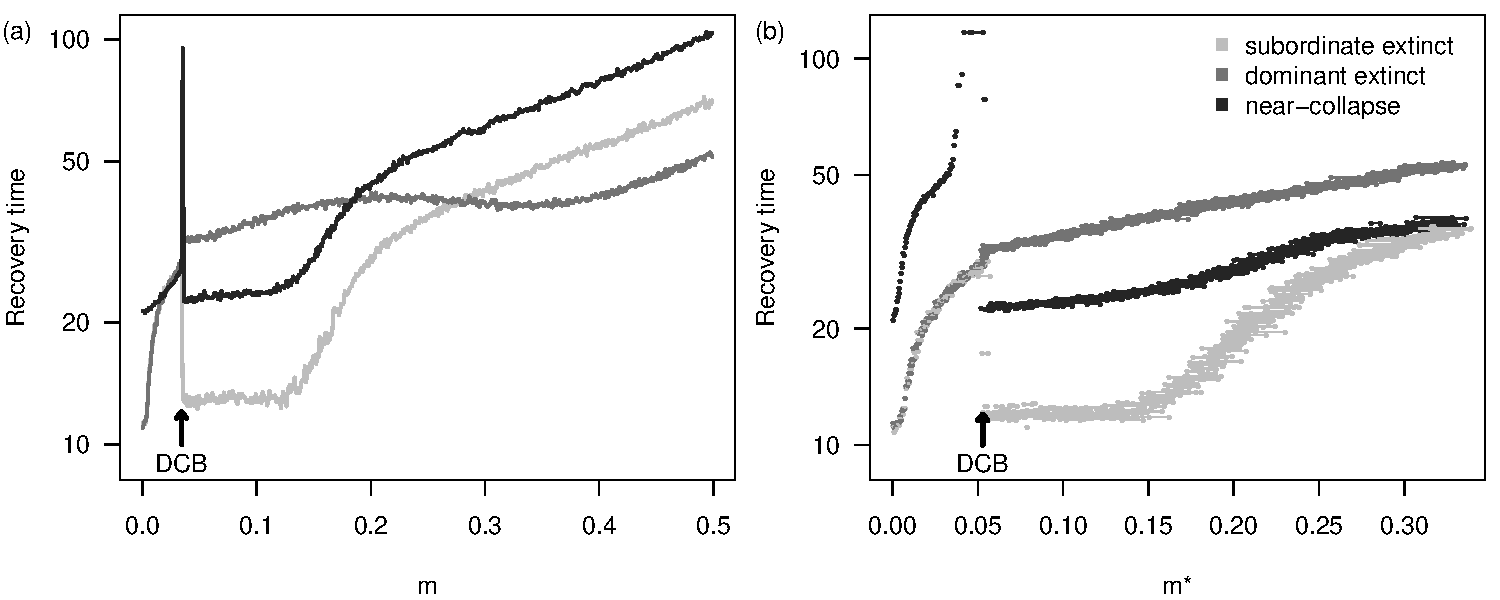
\includegraphics[width=0.9\textwidth]{figs2/fig_relax_lowh.pdf}
\caption{
Recovery time of $N_T$ following the extinction of either the low-density (light gray) or high-density (gray) population, or the near-collapse of both (dark gray) assuming (a) constant straying rates $m$ and (b) density-dependent straying rates (evaluated at the steady state $m^*$) with trait heritability $h^2=0.2$.
If $m$ is density-dependent, in the alternative stable state regime there are two straying rates observed: one each for the low- and high-density populations, respectively, which are linked by a horizontal line.
FB marks the fold bifurcation.
} \label{fig:relax}
\end{figure*}

Trait heritability has a large impact on the degree to which straying rate affects both the aggregate population steady state density ($N^*_T=N^*_1+N^*_2$; figure \ref{fig:PE}a) as well as the difference between steady state densities (the distance between alternative stable states: $\Delta N=|N^*_1-N^*_2|$; figure \ref{fig:PE}b).
Greater trait heritability results in a faster decline in $N_T^*$ with increasing straying rates $m$, but leads to only moderate changes to $\Delta N$.
Conversely, in the context of lower trait heritability, an increase in the straying rate has little impact on the total biomass density but contrastingly large effects on $\Delta N$.
The fold bifurcation (the black line in Figs. \ref{fig:PE}a-c) occurs at lower values of the straying rate $m$ with decreased trait heritability $h^2$ (Fig \ref{fig:PE}a,b), indicating that weaker coupling between ecological and evolutionary dynamics in addition to higher rates of straying promotes the appearance of alternative stable states.
Although trait heritability among salmonids is variable, most life history traits have an $h^2 <0.5$ \cite{Carlson:2008hl}, and we largely focus additional analyses on that range.

%Critical slowing down
As the fold bifurcation is approached with increasing $m$, the portfolio effect increases sharply due to an amplification in variance within both donor and recipient populations.
This amplification in variance is the product of a dynamical process known as \emph{critical slowing down} that occurs near fold bifurcations \cite{Scheffer:2009gg}, a phenomenon that some have suggested may serve as an early warning indicator for approaching phase transitions \cite{Scheffer:2009gg,Lade:2012eu,Anonymous:2013br,Dakos:2014br,Krkosek:2014ch}.
For larger values of $m$ (to the right of the fold bifurcation in Fig \ref{fig:PE}a-c), where alternative stable states occur, the portfolio effect declines steadily as the CV of $N_T$ increases.
The decline over $m$ is more gradual if trait heritability is low, and steeper if trait heritability is high (figure \ref{fig:PE}c).

% \noindent{\bf (c) Rates of recovery following catastrophic collapse}\\ 
% Return time as a measure of system persistence and relation to PE
As the portfolio effect is highly sensitive to the rate of straying between populations, so is the time required for the system to recover to a steady state following a large disturbance.
In general, we find that the average-CV portfolio effect is negatively correlated with recovery time (figure \ref{fig:PE}d), indicating that, for our system, both measures are valuable indicators of metapopulation robustness.
Because we can assess the time to recovery in response to the various disturbance types described above, this allows us to gain an in-depth perspective into the fragility of the metapopulation as a function of straying rate.


Straying had non-linear impacts on the recovery time of populations. 
When the dominant state (well adapted and high density) is wiped out, high levels of straying allow it to recover quickly (figure \ref{fig:relax}a) because the surviving population has a mean trait value skewed towards the optimum of the recovering population (figure \ref{fig:relaxtraj_hdlh}).
Yet, as straying decreases, recovery time for the disturbed dominant state population increases, in part because there is enough time for the trait distribution to move back towards the trait optimum of the subordinate state population.
In contrast, when the subordinate state population (maladapted and low density) is wiped out, recovery rates are fastest at low to intermediate levels of straying.
Because the mean trait values of both populations are skewed towards those of the dominant population, when the subordinate population collapses under high rates of straying, selection against the flood of maladapted individuals that stray into the recovering population extends the length of time required for it to return to its steady state (figure \ref{fig:relaxtraj_ldlh}).
When both populations are both dramatically reduced, recovery time is generally fastest at lower levels of straying, while near the onset of the fold bifurcation, recovery time increases explosively and this is -- as the name implies -- characteristic of \emph{slowing} dynamics that occur near critical transitions \cite{Scheffer:2009gg,Kuehn:2010p2591}.\\


\noindent{\bf (b) The effects of collective migration and density dependent straying} \\
%Portfolio effects
If we assume that the rate of straying is density-dependent, the probability that an individual strays $m_0$ determines the rate of straying within the population, such that $m(t)$ becomes lower as $N(t)$ increases, likely due to the effects of collective decision-making \cite{Berdahl:2016dx} (Eq. \ref{eq:ddm}).
%Because our analyses concern steady state conditions, the inclusion of density-dependent straying does not have a large impact on the qualitative nature of our findings (figure \ref{fig:ddm}).
Density dependence alters the straying rate at steady state population densities because $0 < m^* < m_0$, and this serves to rescale both the strength of the PE as well as the recovery time, but does not change the qualitative nature of our findings.
In the alternative stable state regime, because each population exists at different steady state densities, there are likewise two alternative straying rates $(m_i^*,m_j^*)$: the higher straying rate is associated with the low-density population, and the lower straying rate is associated with the high-density population.
We assessed metapopulation robustness across a range of $(m_i^*,m_j^*)$ values by varying the probability that an individual strays $m_0$, which is positively and linearly related to $(m_i^*,m_j^*)$.
We find that the portfolio effects generated in systems with density-dependent straying are qualitatively similar to systems with constant straying, however there are some important quantitative differences.
First, the PE associated with the high-density (low $m^*$) population is the same as that for a system with a constant $m$ (figure \ref{fig:thetaPE}a).
% As such, the difference in $m^*$ between subordinate and dominant populations appears to matter less than the lower straying rate generated by the dominant population.
As $m^*$ increases, we observe an increase in the PE than for systems with constant $m$.


%Recovery times
Density-dependent straying alters these recovery times (figure \ref{fig:relax}b). 
First, in comparison with constant stray rates, density-dependent straying made recovery more rapid at elevated stray rates when both populations collapsed and when the subordinate population was extirpated.
%Recovery times
%The recovery times for systems with constant and density-dependent straying both show similar trends for a given $m$ and $m^*$ (figure \ref{fig:relax}c,d), however there are some distinct quantitative differences.
At low straying rates, near-collapse of both populations resulted in longer than expected recovery times, whereas in the alternative stable state regime (higher $m^*$), the recovery times for different disturbance types were very similar to systems with a constant $m$ (figure \ref{fig:relax}b; note difference in x-axis scales).
As trait heritability increased, the metapopulation always recovered more quickly if the small population was lost (figure \ref{fig:relax_highh}).
% There was greater similarity in the recovery times for constant and density-dependent $m$ systems when trait heritability was high (figure \ref{fig:relax_highh}).
The lower recovery time for systems with increased $m^*$ mirrors an elevated PE with higher density-dependent straying rates (figure \ref{fig:thetaPE}).
% This higher PE at increased $m^*$ mirrors recovery times that are also lower than those observed for systems with constant $m$ (figure \ref{fig:relax}).
In tandem, analysis of both PE and recovery time suggests that although density-dependent straying does not appear to change the `dynamic landscape' in our minimal model, it does appear to promote robustness, particularly when the aggregate biomass is low and straying is correspondingly high.



\begin{figure}
  \captionsetup{justification=raggedright,
singlelinecheck=false
}
\centering
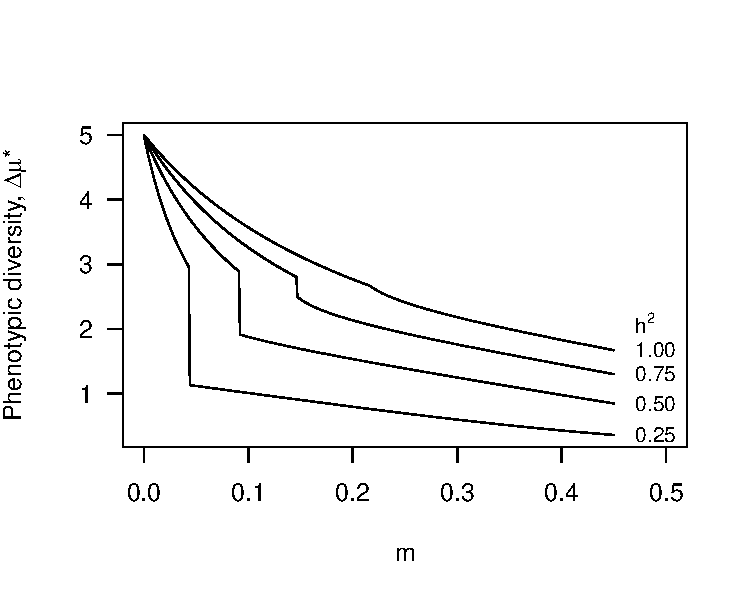
\includegraphics[width=0.5\textwidth]{figs2/fig_traitdiff.pdf}
\caption{
Phenotypic diversity ($\Delta \mu^*$) evaluated at the steady state as a function of straying rate $m$ and trait heritability $h^2$. The descrete jump occurs as the system crosses the fold bifurcation; lower phenoytic diversity emerges with higher straying rates and in the alternative stable state regime. 
} \label{fig:traitdiff}
\end{figure}

%Lowering Phenotypic diversity with increasing straying rate
Increased rates of straying lowers phenotypic diversity ($\Delta \mu^* = |\mu_i(t)-\mu_j(t)|$, evaluated at the steady state) because both local and remote populations are increasingly homogenized.
The loss of phenotypic diversity with increased straying is greater if trait heritability is low because traits take longer to go back to their local optima than they do when heritability is large. 
Hence straying counters the effect of diversifying local adaptation. 
% The loss of phenotypic diversity with increased straying is greater if trait heritability is low because the selective forces acting against trait means far from the local optima are lessened. % with decreased $h^2$.
Less intuitively, we observe a discrete jump towards low phenotypic diversity as the fold bifurcation is crossed (figure \ref{fig:traitdiff}).
Although the development of alternative stable states elevates the portfolio effect due to the variance-dampening effects of the aggregate, entering this dynamic regime also results in a substantial decline in phenotypic diversity, which may have less predictable adverse effects on the population. 
\\


\noindent{\bf (c) The role of habitat heterogeneity and changing selective landscapes}\\ 
\noindent With the onset of straying, we find that increasingly divergent trait optima generally lower $N_T$ and exaggerate $\Delta N$ (figure \ref{fig:thetadiffN}), such that the biomass distribution becomes increasingly uneven. %I've checked this - it's a theshold type (logistic) response Supp fig?
The impact of habitat heterogeneity on the portfolio effect and recovery time is more complex, serving to emphasize the nonlinear relationship between rates of straying and metapopulation robustness. %regardless of heritability.
%The rate of straying that gives rise to a large PE at the fold bifurcation is conditioned on the difference in optimal trait values between the local and remote populations, which we call $\Delta\theta = \sqrt{(\theta_i - \theta_j)^2}$.
As habitat heterogeneity increases, alternative stable states appear at lower straying rates -- with the crossing of the fold bifurcation, accompanied by a peak in the PE -- whereas the magnitude of increase in the PE also increases (figure \ref{fig:thetaPE}b), reducing recovery time (figure \ref{fig:relaxtheta}).
For increased rates of straying, greater habitat heterogeneity erodes the PE (figure \ref{fig:thetaPE}b) and increases the recovery time (figure \ref{fig:relaxtheta}).
These results together suggest that habitat heterogeneity, as measured as the differences in trait optima between two habitats $\Delta\theta$, promotes robustness when straying rates are low, and erodes robustness when straying rates are high.
%This means that alternative stable states can emerge with relatively little dispersal between sites (figure \ref{fig:thetaPE}), however the increased PE (and shorter recovery times).


If we assume that environmental heterogeneity increases with distance between sites, or that individuals may have behaviors that minimize their chances of straying into very different habitats, the rate of straying will decline with habitat heterogeneity.
Accordingly, $\Delta\theta$ will decrease as $m$ increases, such that there are low rates of straying between dissimilar populations and high rates of straying between similar populations.
We find that under these conditions alternative stable states now appear for very low rates of straying $0 < m \leq 0.43$.
As the straying rate increases and $\Delta\theta$ decreases, a single stable state emerges as the fold bifurcation is crossed, which is opposite the pattern observed when these parameters are independent.
There are two notable dynamics that emerge following extinction of the dominant population at low rates of straying between dissimilar (high $\Delta\theta$) sites:
(\emph{i}) above a threshold $m$ value, the dominant population recovers quickly enough that the evolving subordinate phenotype is overwhelmed by incoming strays, and it shifts back to its pre-disturbance (subordinate) state;
(\emph{ii}) below a threshold $m$ value, there is an \emph{inversion} between subordinate and dominant states: because there is enough time and isolation for the subordinate trait mean to shift towards its local optimum, and away from that of the recovering dominant population, the dominant population becomes subordinate, and the subordinate population becomes dominant (figure \ref{fig:inertia}).
This threshold value of $m$, below which the inversion dynamic behavior occurs, is marked by the asterisk in figure \ref{fig:mtheta}, and holds for both constant and density-dependent straying (figure \ref{fig:mthetamvm}).

% At low rates of straying, there is little mixing between dissimilar populations, and this leads to the formation of alternative stable states.
% Here we find that if the subordinate population is wiped out, the time to recovery is minimized, whereas if the dominant population is wiped out, the time to recovery is maximized; near-collapse of both results in intermediate recovery times.
% When straying rates are low and the difference in trait optima are correspondingly high, we might assume that extinction of the dominant population would result in relatively faster recovery.
% This would be a logical assumption because the mean trait value of the subordinate population would be skewed towards that of the dominant (larger) population, such that recruitment at the disturbed site should be high and the population should recovery more quickly.
% Our results show, however, that \emph{this assumption is wrong:} although the mean trait value of the subordinate population \emph{is} skewed towards the optimum of the dominant population, when the latter is wiped out and the rate of straying is low, there is enough time and isolation for the subordinate trait mean to shift towards its own optimum, and away from that of the recovering dominant population (figure \ref{fig:inertia}).
% This \emph{selective inertia} occurs until the dominant population grows large enough that the evolving subordinate phenotype is overwhelmed by incoming strays, shifting it back to its pre-disturbance (subordinate) state.
% This effect can lead to much longer recovery times for the dominant population.
% Importantly, if the rate of straying is below a threshold value, it can also result in a state-switch, wherein increased isolation permits the subordinate population to \emph{escape} the selective pull of the dominant population, leading to a switching in which population is in the dominant/subordinate state.



\begin{figure}
  \captionsetup{justification=raggedright,
singlelinecheck=false
}
  \centering
  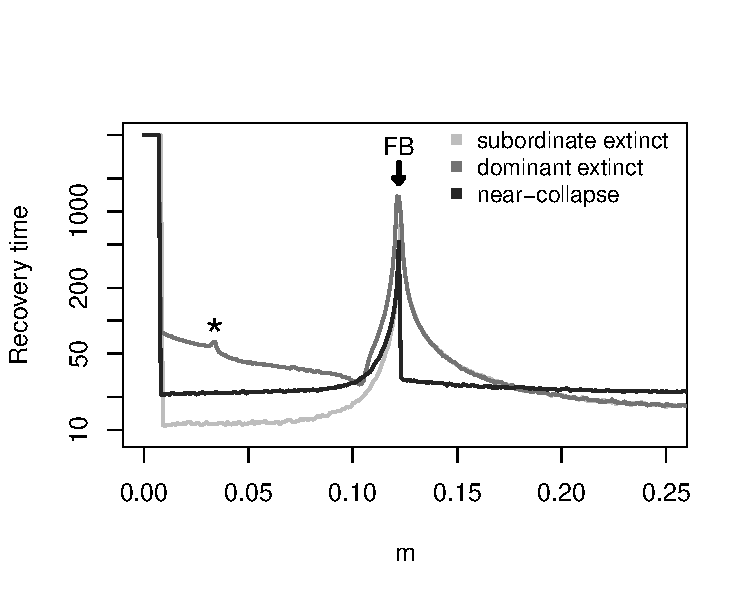
\includegraphics[width=0.5\textwidth]{figs2/fig_mtheta_rt.pdf}
  \caption{
  Distance dependent recovery times for three disturbance types. When straying is distance dependent, $m$ increases as $\Delta\theta$ decreases.
  The `$*$' marks the value of $(m,\Delta\theta)$ below which there is a switch in subordinate/dominant states following extinction of the dominant population.
  FB marks the fold bifurcation.
  } \label{fig:mtheta}
\end{figure}



% That alternative stable states appear and that PE becomes severely depressed for very low rates of straying is surprising: this means that even a small amount of mixing of populations from distant or dissimilar populations can qualitatively alter the dynamics of the metapopulation, regardless of trait heritability.
%(for the discussion: an example of this situation may be the salmon populations during the last glacial maximum, where any mixing would be from geographically distant populations)



\section{Discussion}

We have shown that density-dependent straying between populations consistent with collective navigation, coupled with localized selection against donor phenotypes, has a large and nonlinear impact on dynamic properties that affect metapopulation robustness.
We measured robustness as:
1) the average-CV portfolio effect \cite{Anderson:2013gb,Anonymous:2015gf}, a statistical metric commonly used to assess the buffering capacity of metapopulations, and
2) the recovery time, defined here as the time required for the aggregate metapopulation biomass $N_T$ to return to its steady state following an induced disturbance, which is mechanistically linked to persistence \cite{Ovaskainen:2002il}.
In our minimal eco-evolutionary model of dispersal and natural selection between two populations, we show that these statistical and mechanistic descriptors of metapopulation dynamics and robustness are tightly coupled (figure \ref{fig:PE}d), which is not uncommon for diverse metrics of stability \cite{Donohue:2013iu}.
Taken as a whole, our results point to an important role of density-dependent straying in the colonization and recovery dynamics within metapopulations, while also underscoring the risk of straying by individuals with maladaptive traits to reduce the productivity of locally adapted stock complexes.

% 
% %The bifurcation and critical slowing down
% [This paragraph is interesting to me but could be cut] Although the portfolio effect is negatively correlated with recovery time, there is one exception: the point of transition from a single steady state to alternative stable states, which occurs at the fold bifurcation (REF).
% At this point, the portfolio effect is maximized, but so is the recovery time (figures \ref{fig:PE}, \ref{fig:relax}).
% This suggests that while the sharply increasing variance of the individual populations is dampened by aggregation, a large disturbance will have a much greater adverse effect due to exponentially longer recovery times.
% Whether the change in variance, also known as critical slowing down, as the alternative stable state regime is approached could be used as an early warning signal of an oncoming phase transition is a hotly debated topic (REFS).
% The detectability of such changes in dynamical behavior among salmonids appears to be idiosyncratic across species, though the difficulty in measuring critical slowing down may - ironically - be masked by large portfolio effects \cite{Krkosek:2014ch}.
% 

%alternative stable states & critical slowing
A salient finding from our results was that straying can lead to the emergence of alternative stable states, pushing one of the populations to high density (the \emph{dominant state}), and one to low density (the \emph{subordinate population}).
This asymmetry in population densities also leads to an asymmetry in the mean trait values, both of which are skewed towards the local optimum of the dominant population. 
The formation of alternative stable states in our system is a relatively common example of spatial pattern formation. %, only occurring above a threshold straying rate that largely depends on trait heritability and the difference in trait optima between sites.
Pattern formation can occur as a consequence of myriad ecological processes, including habitat selection, aggregation, local environmental conditions, and/or interspecific interactions such as competition or predation, and is inexorably linked to scale \cite{Levin:1992p1472}. 
Pattern formation is also known to occur with the onset of spatially or diffusion-induced instabilities, or Turing instabilities \cite{Meinhardt:2012hw}. 
Here, we describe an additional mechanism by which pattern formation in local densities can occur, when the onset of collective movement-mediated maladaptation leads to local differences in reproductive rates resulting in alternative stable states across sites. 
%This mechanism of pattern formation through the simultaneous interplay between ecological and evolutionary dynamics may open up new areas of research.
While metapopulation approaches have widely recognized the importance of source and sink populations \cite{Hanski:1999vu} as well as the occurrence of alternative states \cite{Boughton:1999fa}, here we show that the coupled forces of ecological and evolutionary processes can result in similar populations diverging into alternative states where one population is large and well-adapted, while the other is smaller and maladapted.
The appearance of these alternative states is largely dependent on the dispersal, or rate of straying, between sites.

% 
% To what extent the existence of alternative stable states promotes or diminishes the system as a whole is a matter of perspective, though with clear conservation implications.
% At face value, the subordinate population is pushed closer to extinction (figure \ref{fig:traj}), suggesting that the system may be more fragile.
% On the other hand, the presence of \emph{just enough} straying to cause formation of alternative stable states both increases the portfolio effect (figure \ref{fig:PE}c) and reduces the rate of return -- particularly if straying is density-dependent (figures \ref{thetaPE}a, \ref{fig:relax}b).
% This asymmetry in population densities also leads an asymmetry in the mean trait values, skewed towards the local optimum of the dominant population, one, and this has important -- and often non-intuitive -- ramifications for metapopulation robustness. %, as measured by both the portfolio effect as well as recovery time.

There is a `sweet spot' for straying that maximizes metapopulation robustness. 
Results from our model reveal that the presence of just enough straying to cause formation of alternative stable states increases the portfolio effect (figure \ref{fig:PE}a). 
Previous theoretical work has shown that increased connectivity may erode portfolio effects in herring metapopulations, where straying is also thought to be density-dependent \cite{Secor:2009ena}.
Although high levels of dispersal in our system generally supports this finding, the interplay between dispersal and PE is more subtle when selection for local adaptations is considered, such that low to intermediate levels of density-dependent straying result in an elevated PE, thus increasing the buffering capacity of the metapopulation.
Although PE is measured at the steady state, low to intermediate rates of straying also appear to have a beneficial effect on transient dynamics.
When there is just enough straying to cause alternative stable states, the time to recovery following an induced disturbance declines, though -- as with the PE -- recovery time then grows if straying becomes very large (figure \ref{fig:relax}a).

% %Density dependent straying
% This themed issue is largely concerned with the notion that straying in biological systems where movement is a function of collective navigation may be density-dependent.
% Berdahl et al. (REF) provided a mechanistic hypothesis for density-dependent straying where the proportion of the population that strays is less than the probability that a single individual takes the wrong turn. %(as illustrated by \emph{Kevin}; figure \ref{fig:xkcd}) takes the wrong turn.
% Neither the transient nor asymptotic dynamics that we describe here qualitatively differ as a function of whether the rate of straying is constant or density-dependent, however we observe important quantitative differences that suggest density-dependent straying may play an important role in the persistence of metapopulations over evolutionary time.

This themed issue formalizes the role of collective movement in the ecology of natural systems and illuminates a signature of collective navigation in animal populations on the move.
We observed three salient results that contribute to our understanding of collective movement that combine to suggest that density-dependent straying may play an important role in the persistence of metapopulations over evolutionary time.
First, the inclusion of density-dependent straying does not qualitatively alter either (\emph{i}) steady state or (\emph{ii}) transient dynamics of our minimal eco-evolutionary model, but effectively rescales measures of robustness to the lower straying rates that emerge as a consequence of the coupled dynamics.
Second, compared to systems with constant dispersal, density-dependent straying appears to increase the portfolio effect across a range of straying rates (figure \ref{fig:thetaPE}a). 
% and that at low to intermediate levels of straying, PE is high.
Third, density-dependent straying reduces the time to recovery following disturbance, and this is particularly true in the case of near-collapse of the metapopulation (figure \ref{fig:relax}b).
In the case of near-collapse, although both populations inherit low population densities, the mean trait values of both are skewed towards the optimum of the dominant population.
Due to density-dependent straying, low population densities evince greater dispersal, and while this increased connectivity primarily facilities the growth of the dominant population (because the trait means are closer to the dominant optimum), because the dominant population contains the bulk of the aggregate biomass, the overall recovery time is lessened significantly (figures \ref{fig:relax}b, \ref{fig:relaxtraj_bothlh}).
% Third, in habitats with greater heterogeneity between sites (measured by an increase in $\Delta\theta$), density-dependent straying diminished robustness at low rates of straying (marginally lower portfolio effects and substantially longer return times; figures \ref{fig:thetaPE}b, \ref{fig:relaxtheta}a,b).
% Conversely, for increased straying rates, greater and exaggerates the positive effects when $m^*$ is high (higher portfolio effects, and shorter return times). 



% %Comparing recovery times
% Previous theoretical work has shown that the largest perturbations lead to the longest recovery times \cite{Ovaskainen:2002il}.
% In terms of relative biomass lost, the largest perturbation that we investigate is the near-collapse of both populations, where only 1\% of the pre-perturbation densities survive, however whether this disturbance results in the longest recovery time depends largely on the rate of straying and trait heritability.
% For example, when straying and trait heritability are low (figure \ref{fig:relax}) the extinction of the larger population maximizes return times, whereas if straying is high, near-collapse maximizes return time.
% The latter is always true in the alternative stable state regime if trait heritability is high (figure \ref{fig:relax_highh}).

%Habitats 
Salmon are distributed and stray across a diverse range of habitats, and the rates of straying between geographically diverse sites can be plastic and idiosyncratic \cite{Westley:2015to}.
Our surrogate measure for habitat heterogeneity is the difference in trait optima between sites $\Delta\theta$.
In general, our findings indicate that increased habitat heterogeneity promotes robustness (higher PE, shorter time to recovery) when straying rates are low, but may erode robustness when straying rates are high (figure \ref{fig:thetaPE}b, solid lines).
This may be particularly consequential for populations that are spatially adjacent but separated by sharp environmental boundaries, such that trait optima are divergent yet dispersal is relatively high.
Such a scenario plays out repeatedly in the context of adjacent wild and hatchery-produced salmon. 
Although wild and hatchery populations may occur close on the landscape, and indeed often are sympatric within the same river network, the selective environments to which they are locally adapted differ dramatically \cite{Christie:2012bj}. 
Straying of domesticated hatchery-produced fish from release sites and spawning in the wild drastically reduces the productivity of wild populations through competition and outbreeding depression \cite{Chilcote:2003bb,Araki:2007cm}.

%mtheta
All else being equal, habitats that are closer in space generally have greater similarity in environmental conditions than habitats that are geographically distant, and correspondingly phenotypes of more proximately located populations should be more similar to those that are distant \cite{Westley:2012ui}.
It is thus reasonable to expect a larger number of straying individuals between sites that are geographically proximate and indeed evidence corroborates this prediction \cite{Candy:2000hu,JPE:JPE1383}.
Alternatively, salmon that cue to specific environmental conditions may be more likely to stray into sites that have structurally and physiognamically similar habitats \cite{Peterson:2014gy} even if other potential sites are closer.
These considerations justify imposing a direct relationship between the rate of straying $m$ and habitat heterogeneity: as site dissimilarity increases, so too should the straying rate decrease.
% As site dissimilarity increases, so to should the optima in trait values for the resident populations.
When habitat heterogeneity and the rate of straying are linked in this way, we show that very small amounts of either constant or density-dependent straying result in long recovery times for the dominant population because there is time for selection to push the subordinate trait mean away from the optimum of the dominant population (figure \ref{fig:mtheta}). %there is enough isolation to allow the surviving subordinate population to adapt towards its own optimum.
If the straying rate is very low, there is an inversion in the alternative stable states following the disturbance, resulting in a state shift in dominance.
This may have particular conservation implications for considerations of aiding dispersal following disturbances or reconnections of lost habitats \cite{Anderson:2013bf,Pess:2014isa}.
% Moreover, local temperature regimes are known to play a central role in dictating local adaptation of salmon populations.
% If temperature is the primary determinant of $\Delta\theta$ in terms of our model, this would suggest that populations spanning North-South gradients are more predisposed to distance dependent dynamics.
% In contrast, the relationship between the rate of straying and habitat heterogeneity may be less clear-cut for populations spanning an East-West gradient, where distant habitats may equally fitting for straying populations.


% Our model is a simple framework for an initial consideration of the eco-evolutionary dynamics of metapopulation and accordingly made assumptions that are important to clarify. 
% First, our model did not consider the role of straying and dispersal in introducing new genetic material that can combat genetic challenges of small populations such as inbreeding. 
% Second, our model did not incorporate the potential genetic underpinnings of response diversity and asynchrony. 
% We anticipate that including a link between genetic divergence and population stochasticity would exacerbate the rate at which higher straying would synchronize populations. 
% Third, our model assumed that strays were incorporated into the trait distribution of the recipient populations—in natural systems it is possible that strays may die prior to reproduction when the two habitats are highly divergent. 
% Fourth, natural systems are quite temporally? variable, which could push systems out of steady-state dynamics, which is what our model focused on. 
% Fifth, we focused on an extremely simple system of two linked populations. While more linked populations would introduce additional complexity, we predict that our qualitative results would apply to more complicated systems. 
% It is clear that understanding the eco-evolutionary dynamics of metapopulations is a rich area for further research.


Although our study was inspired by salmon metapopulations, the results have general implications for the conservation and management of other migratory metapopulations as well. 
Because changes in straying rates can have large and nonlinear impacts on robustness, human activities that alter straying rates could have unintended consequences. 
For example, salmon produced by hatcheries often stray into proximate wild populations \cite{Brenner:2012gl}, and these recipient populations can have lower fitness due in part to the introduction of maladapted genes \cite{Ford:2002ip}. 
We show that there is an intermediate straying rate where disturbed populations that are recovering by the introduction of maladapted strays recover fastest: if the straying rate is too low or too high, recovery times increase (figure \ref{fig:relax}).
This finding suggests that salmon stocking efforts that aim to lower recovery times following dam removal could actually prolong recovery if the rate at which individuals are introduced is not taken into account.
Ongoing examinations of experimental restocking in the recently re-opened Elwha River (Washington State) will provide empirical insight into the potential short- and long-term consequences of facilitated recovery \cite{Liermann:2017gj}. 

% More generally, the current attributes and resilience of salmon metapopulations are likely a function of their history of evolving in dynamic river systems that periodically experienced massive disturbances such as landslides, glaciers, and floods over different climatic regimes (Waples et al. 2009; Waples et al. 2008). 
% Population declines following these disturbances would also magnify the rate of straying, and our results suggest that this response in the straying rate would quicken the recovery of the small populations that survive.
% Indeed, we found that density-dependent migration appears to increase the robustness of metapopulations faced with large-scale disturbance, particularly in regimes where populations have lower steady states and correspondingly higher rates of straying.
% As population numbers increase and stray rates decrease, the metapopulation could achieve higher production due to fine-scale local adaptation unhindered by high rates of maladaptive strays. 

The portfolio effect and the time to recovery following a disturbance are independent and correlated measures of metapopulation robustness that take into account both steady state and transient dynamics.
We show that these measures of robustness are strongly influenced by the rate at which individuals from donor populations stray into habitats occupied by recipient populations. 
Importantly, density-dependent straying, which may occur when individuals collectively navigate, can both increase the portfolio effect and lower the time to recovery following a disturbance, which is anticipated to promote persistence. 
We suggest that understanding the spatial complexity of metapopulations dispersing across heterogeneous environments, in tandem with the mosaic of selective forces acting on those environments, may be key to uncovering those factors that promote persistence in the wild.




% 
% 
% %Concluding
% The importance of selection and its influence on the dynamics of populations is increasingly recognized as vital for assessing species' fragility.
% Of particular interest is how selection might influence spatially coupled metapopulations distributed across environmental gradients.
% We have shown that two measures of metapopulation robustness -- the portfolio effect and the time to recovery following a disturbance -- are strongly influenced by the rate at which individuals from a donor population stray into habitats occupied by a recipient population.
% Importantly, density-dependent straying, which may occur when individuals collectively navigate, can both increase the portfolio and lower the time to recovery following a disturbance, which is anticipated to promote persistence.
% We suggest that understanding the spatial complexity of metapopulations dispersing across heterogeneous environments, combined with the mosaic of selective forces acting on those environments, may be key to discovering those factors that promote persistence.


\bibliography{aa_kevin}


\beginsupplement


\begin{figure}
  \captionsetup{justification=raggedright,
singlelinecheck=false
}
\centering
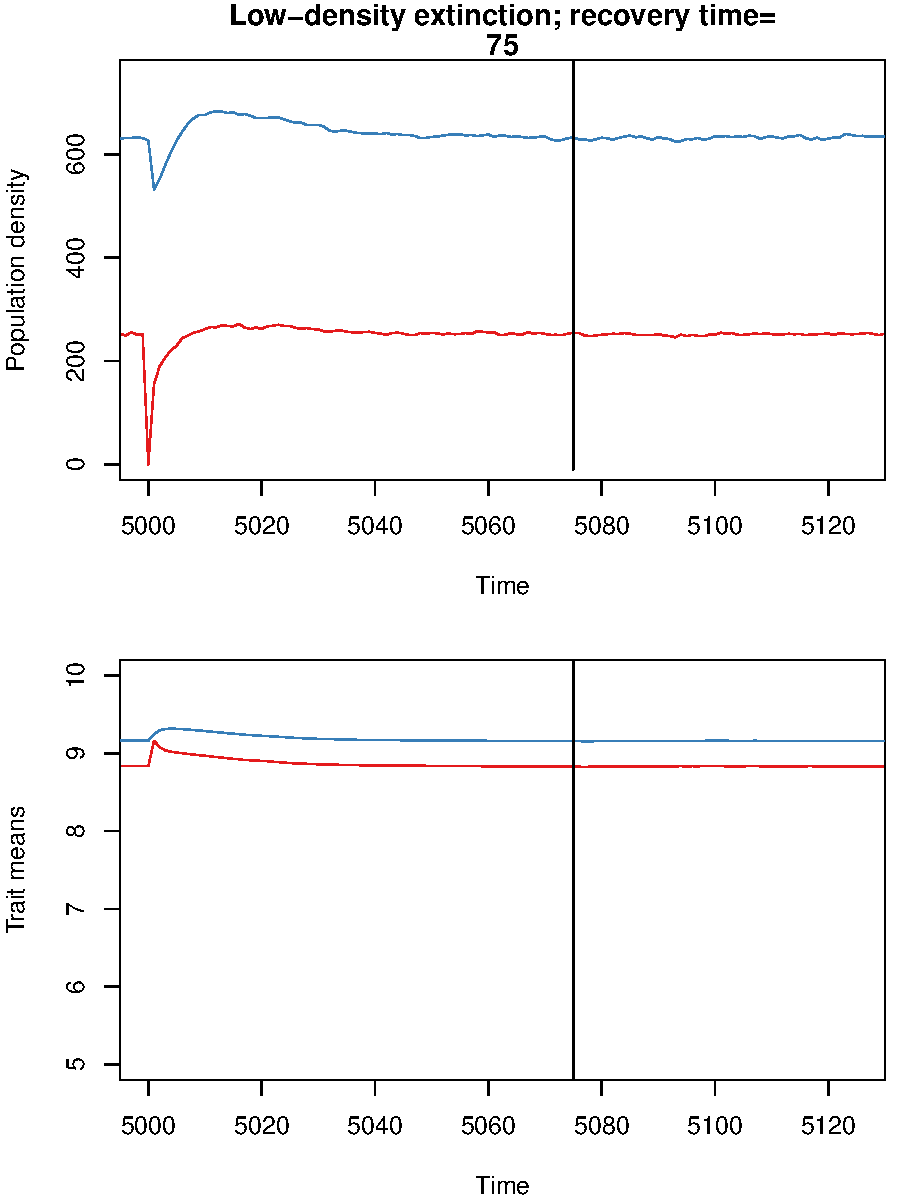
\includegraphics[width=0.35\textwidth]{figs2/fig_relax_small.pdf}
\caption{
Extinction of low-density population with a high constant straying rate $m=0.4$ and low trait heritability $h^2=0.2$ (see figure \ref{fig:relax}a).
Black line marks the calculated point of recovery post-perturbation.
Trait optima are $\theta_1 = 10$ (blue population trajectory) and $\theta_2 = 5$ (red population).
} \label{fig:relaxtraj_ldlh}
\end{figure}

\begin{figure}
  \captionsetup{justification=raggedright,
singlelinecheck=false
}
\centering
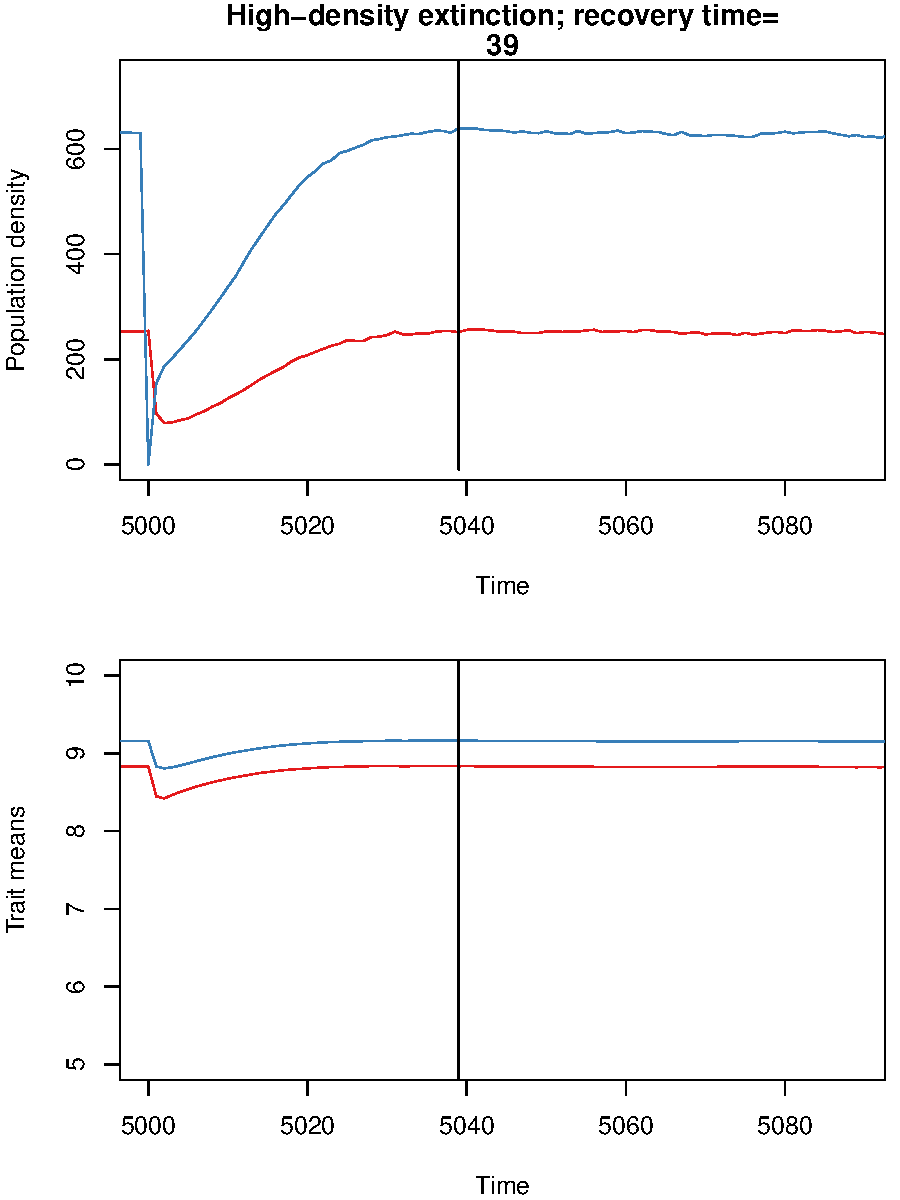
\includegraphics[width=0.35\textwidth]{figs2/fig_relax_large.pdf}
\caption{
Extinction of high-density population with a high straying rate $m=0.4$ and low trait heritability $h^2=0.2$ (see figure \ref{fig:relax}a).
Black line marks the calculated point of recovery post-perturbation.
Trait optima are $\theta_1 = 10$ (blue population trajectory) and $\theta_2 = 5$ (red population).
} \label{fig:relaxtraj_hdlh}
\end{figure}
% 
% \begin{figure}
%   \captionsetup{justification=raggedright,
% singlelinecheck=false
% }
% \centering
% 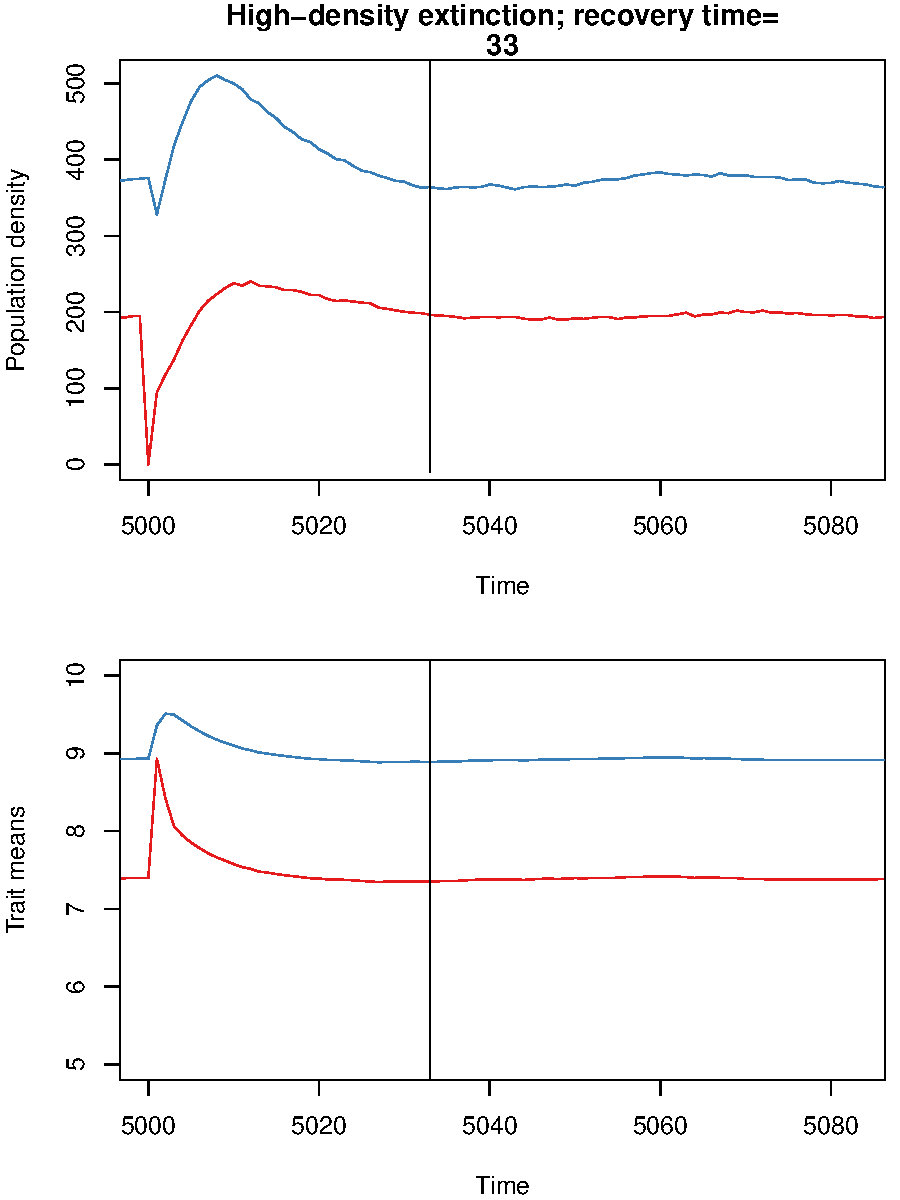
\includegraphics[width=0.35\textwidth]{figs2/fig_relax_small_highh.pdf}
% \caption{
% Extinction of low-density population with a high constant straying rate $m=0.4$ and high trait heritability $h^2=0.8$ (see figure \ref{fig:relax}a).
% Black line marks the calculated point of recovery post-perturbation.
% Trait optima are $\theta_1 = 10$ (blue population trajectory) and $\theta_2 = 5$ (red population).
% } \label{fig:relaxtraj_ldhh}
% \end{figure}
% 
% \begin{figure}
%   \captionsetup{justification=raggedright,
% singlelinecheck=false
% }
% \centering
% 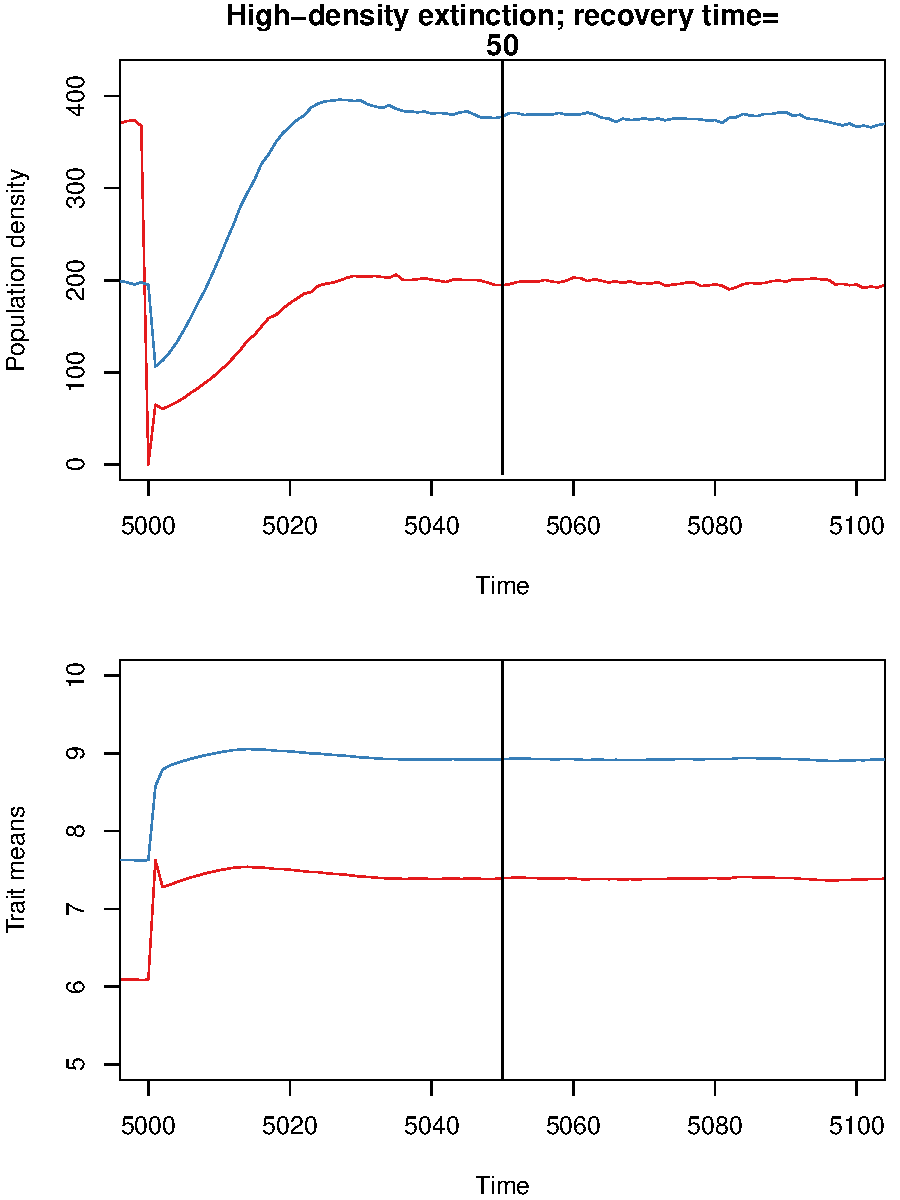
\includegraphics[width=0.35\textwidth]{figs2/fig_relax_large_highh.pdf}
% \caption{
% Extinction of high-density population with a high straying rate $m=0.4$ and high trait heritability $h^2=0.8$ (see figure \ref{fig:relax}a).
% Black line marks the calculated point of recovery post-perturbation.
% Trait optima are $\theta_1 = 10$ (blue population trajectory) and $\theta_2 = 5$ (red population).
% } \label{fig:relaxtraj_hdhh}
% \end{figure}

\begin{figure*}
  \captionsetup{justification=raggedright,
singlelinecheck=false
}
\centering
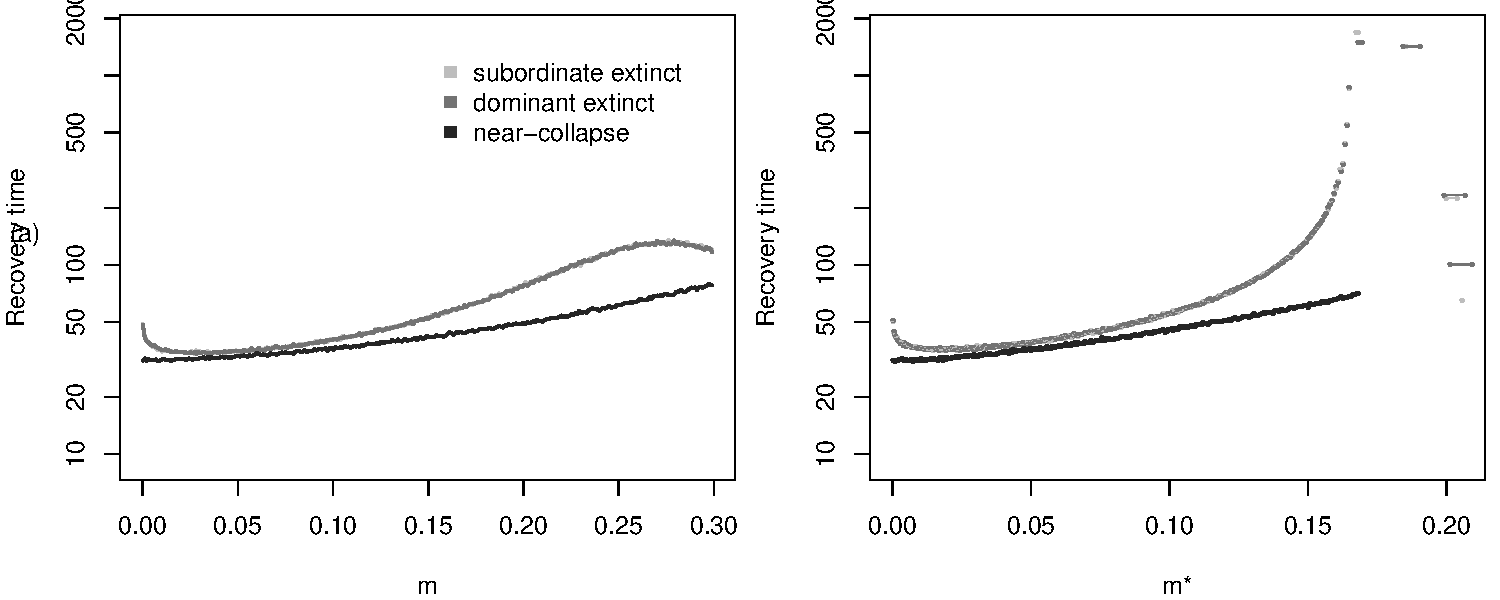
\includegraphics[width=0.9\textwidth]{figs2/fig_relax_highh.pdf}
\caption{
Recovery time of $N_T$ following the extinction of either the low-density (light gray) or high-density (gray) population, or the near-collapse of both (dark gray) assuming (a) constant straying rates $m$ and (b) density-dependent straying rates (evaluated at the steady state $m^*$) with trait heritability $h^2=0.8$.
If $m$ is density-dependent, in the alternative stable state regime there are two straying rates observed: one each for the low- and high-density populations, respectively, which are linked by a horizontal line.
} \label{fig:relax_highh}
\end{figure*}



\begin{figure}
  \captionsetup{justification=raggedright,
singlelinecheck=false
}
\centering
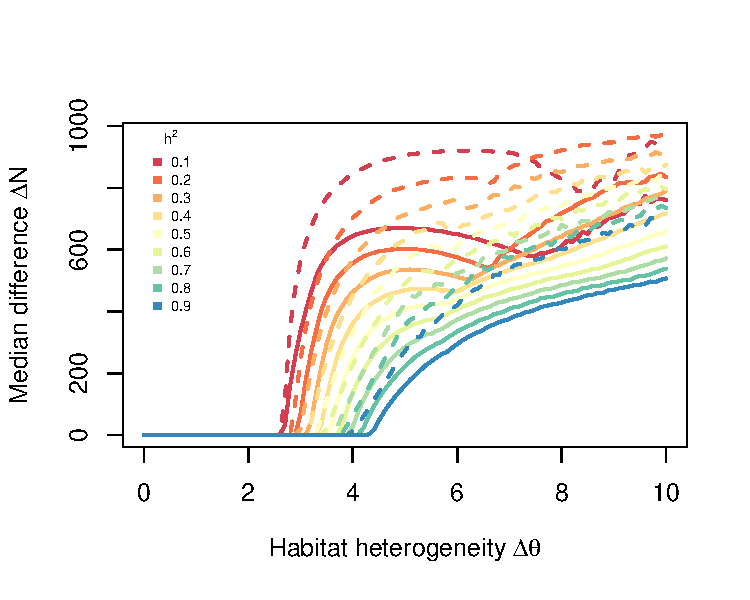
\includegraphics[width=0.4\textwidth]{figs2/fig_thetadiffN.pdf}
\caption{
Median difference in population densities taken over the straying rate as a function of habitat heterogeneity $\Delta\theta$.
Solid lines are for constant $m$; dashed lines are for density-dependent $m$} \label{fig:thetadiffN}
\end{figure}



\begin{figure*}
  \captionsetup{justification=raggedright,
singlelinecheck=false
}
\centering
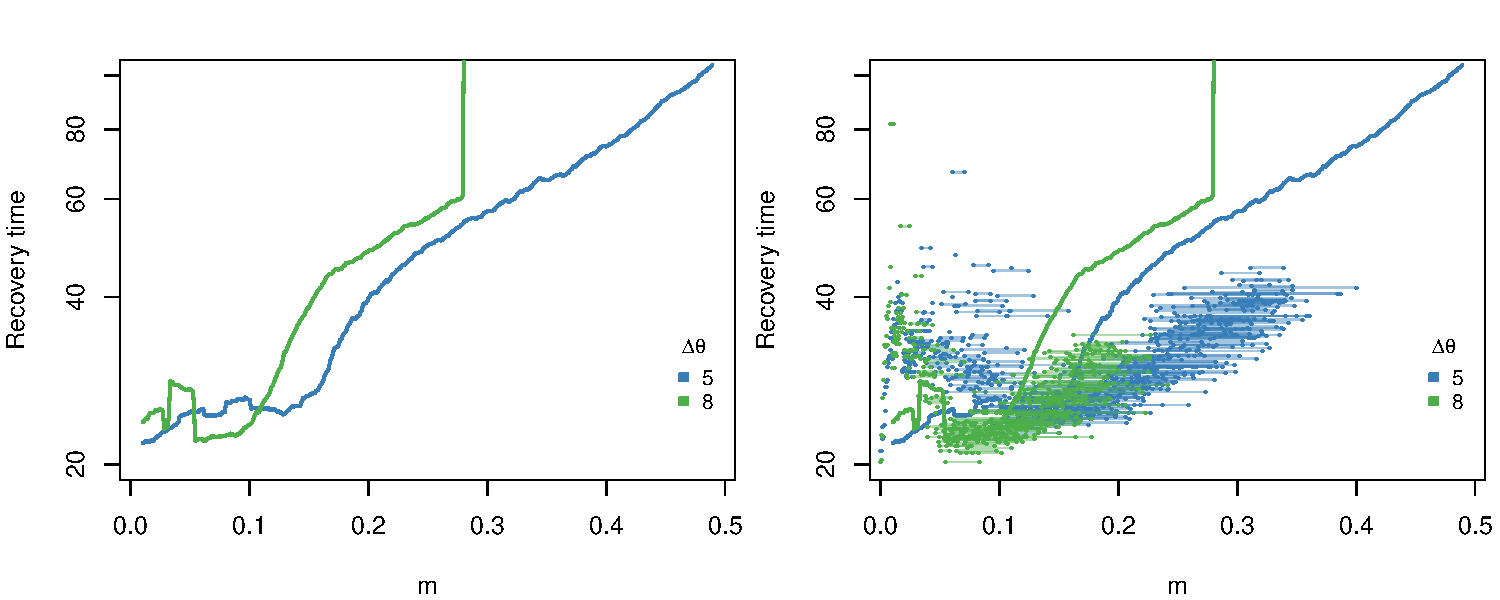
\includegraphics[width=0.8\textwidth]{figs2/fig_relaxtheta2.pdf}
\caption{
(a) Recovery time after near collapse of both populations as a function of straying rate $m$ and habitat heterogeneity $\Delta\theta$.
(b) The same as (a) but including recovery times when straying is density-dependent, shown by linked pairs of points.
Recovery times for systems with density-dependent straying are longer at low straying rates and shorter at higher straying rates, mirroring the change in portfolio effects shown in figure \ref{fig:thetaPE}.
} \label{fig:relaxtheta}
\end{figure*}


\begin{figure}
  \captionsetup{justification=raggedright,
singlelinecheck=false
}
  \centering
  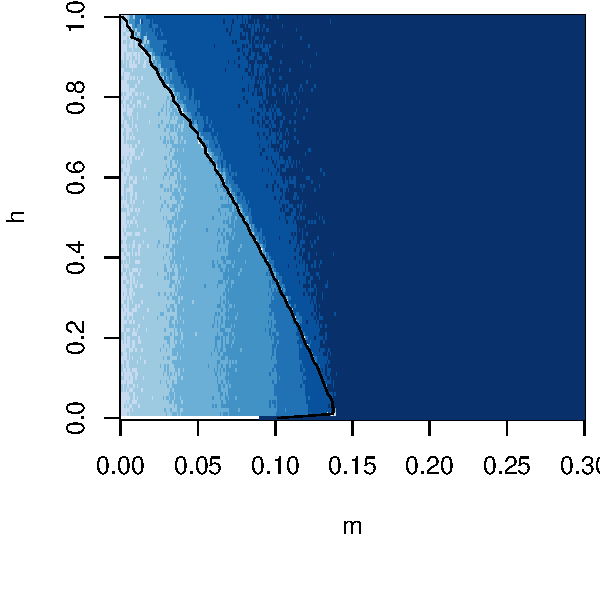
\includegraphics[width=0.35\textwidth]{figs2/fig_MDPE_hm_mtheta_rt.pdf}
  \caption{
  Distance dependent portfolio effects as a function of straying rate $m$ and trait heritability $h^2$. When straying is distance dependent, $m$ increases as $\Delta\theta$ decreases.
  } \label{fig:mthetaPE}
\end{figure}

\begin{figure}
  \captionsetup{justification=raggedright,
singlelinecheck=false
}
\centering
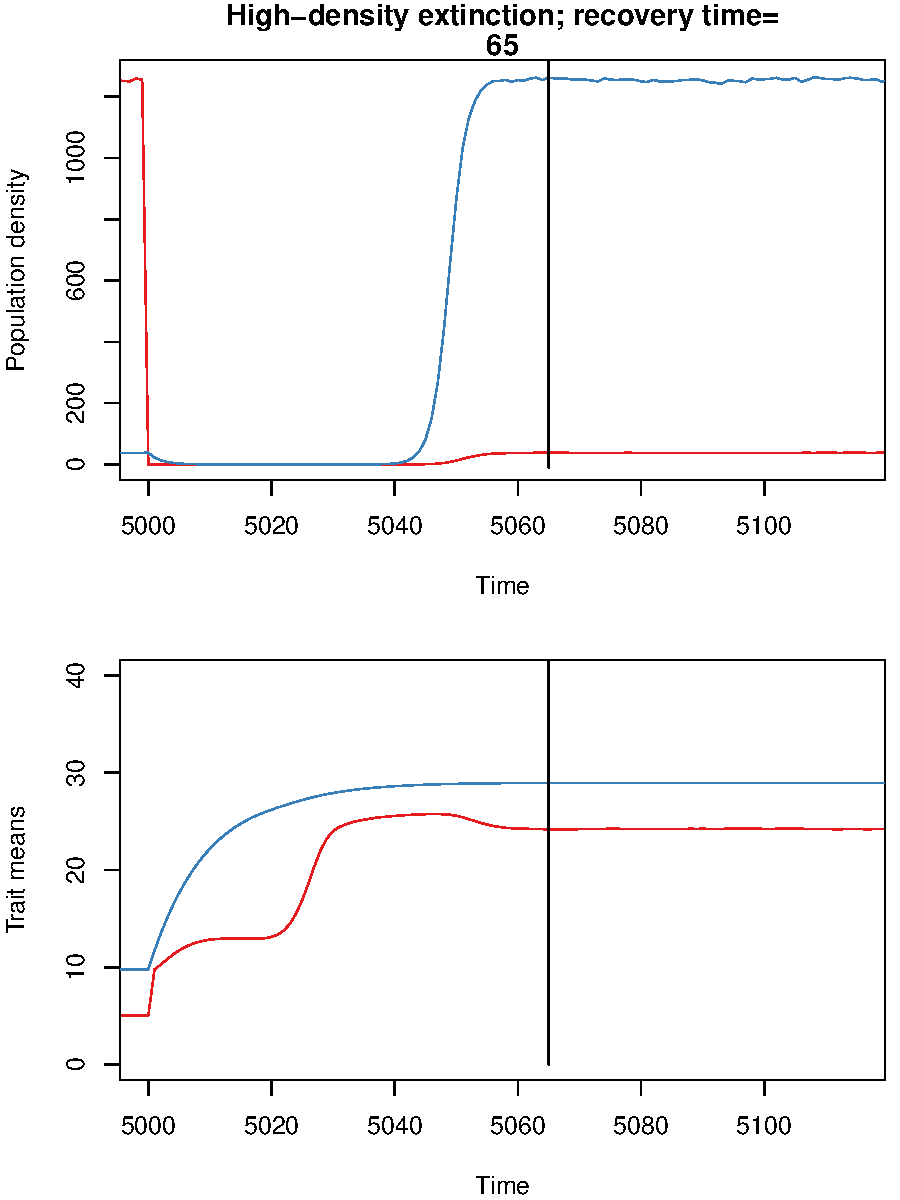
\includegraphics[width=0.35\textwidth]{figs2/fig_relax_inertia.pdf}
\caption{
Distance dependent straying, where increased differences in trait optima between sites $\Delta\theta$ corresponds to lower rates of straying $m$.
At low rates of straying $m=0.02$ ($\Delta\theta=24$), extinction of the dominant population leads to slower-than-expected recovery times because the subordinate population is isolated enough to evolve towards its own trait optimum. %until growth of the dominant population overwhelms this local selection.
In this case, $m$ is less than $m=0.034$ (denoted by the asterisk in figure \ref{fig:mtheta}), such that isolation allows the subdominant population to `run away' from the influence of the dominant population, leading to a switch in states.
If $m$ is low but greater than $0.034$, isolation permits the subdominant population to `run away' from the influence of the dominant population, until it is overwhelmed by the recovering dominant population, and reverts back to its previous trait mean prior to the disturbance.
} \label{fig:inertia}
\end{figure}

\begin{figure*}
  \captionsetup{justification=raggedright,
singlelinecheck=false
}
  \centering
  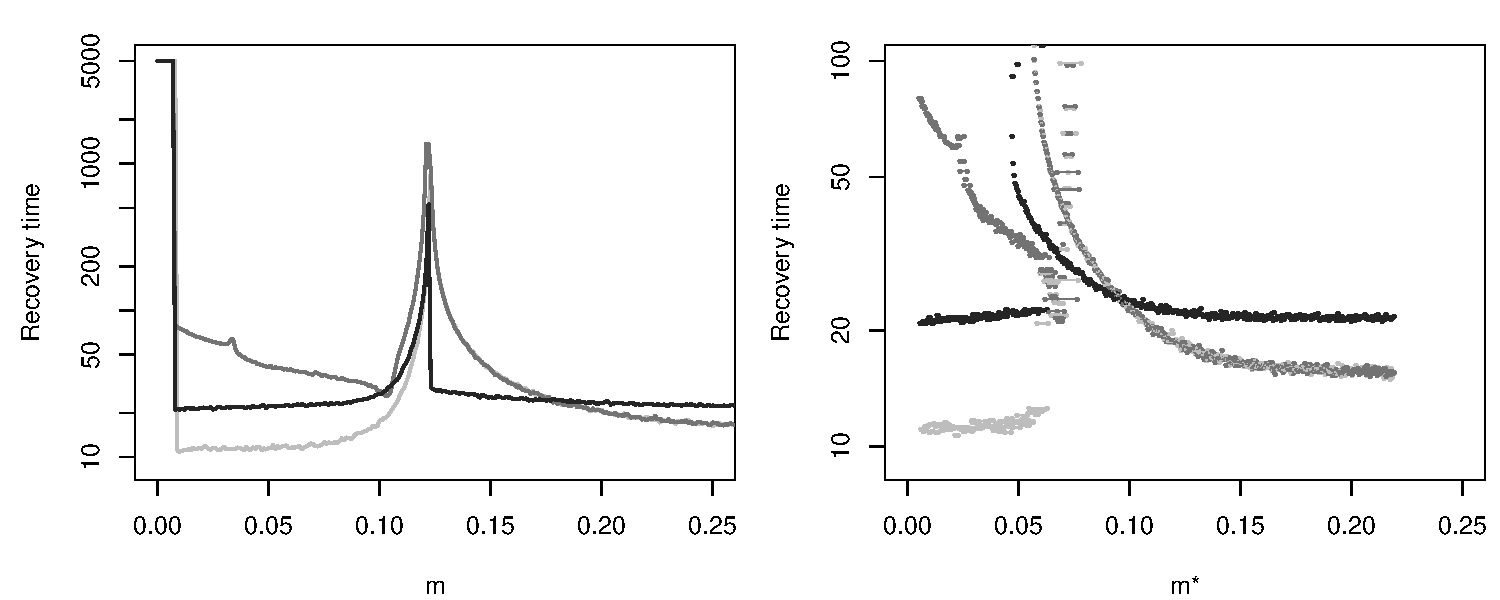
\includegraphics[width=0.8\textwidth]{figs2/fig_relax_mtheta.pdf}
  \caption{
  Distance dependent recovery times for three disturbance types. When straying is distance dependent, $m$ increases as $\Delta\theta$ decreases for constant (a) and density-dependent (b) staying rates.
  The fold bifurcation is not as clear in (b) because $\Delta\theta$ is a function of the individual straying rate $m_0$, whereas the x-axis in (b) is the straying rate at the steady state $m^*$.
  Despite this difference, the general trends shown in (a) are also present in (b).
  } \label{fig:mthetamvm}
\end{figure*}



\begin{figure}
  \captionsetup{justification=raggedright,
singlelinecheck=false
}
\centering
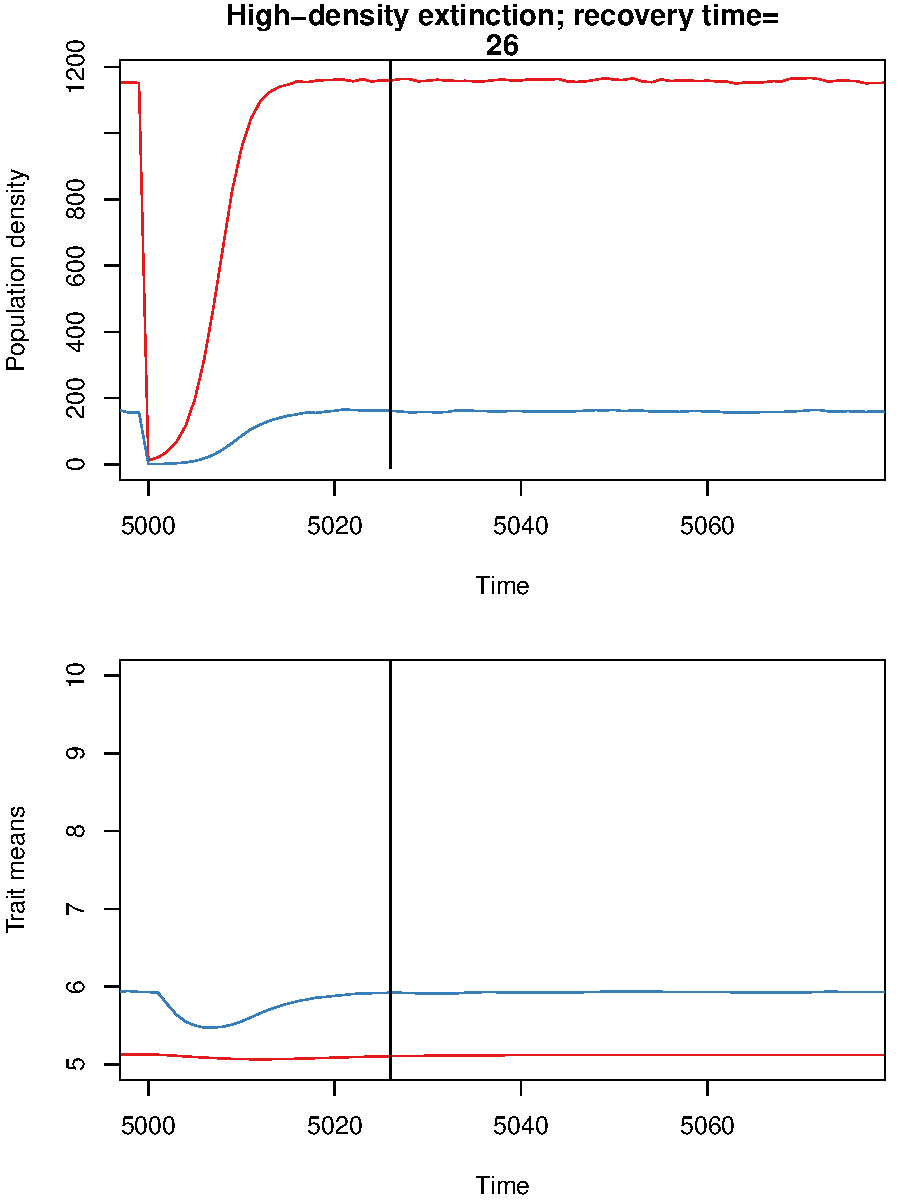
\includegraphics[width=0.35\textwidth]{figs2/fig_relax_both_lowh.pdf}
\caption{
Near collapse of both populations with a low straying rate $m=0.1$ and low trait heritability $h^2=0.2$ (see figure \ref{fig:relax}a).
Black line marks the calculated point of recovery post-perturbation.
Trait optima are $\theta_1 = 10$ (blue population trajectory) and $\theta_2 = 5$ (red population).
} \label{fig:relaxtraj_bothlh}
\end{figure}


% \begin{figure*}[h!]
%   \captionsetup{justification=raggedright,
% singlelinecheck=false
% }
% \centering
% \begin{subfigure}[t]{0.55\textwidth}
% \centering
% 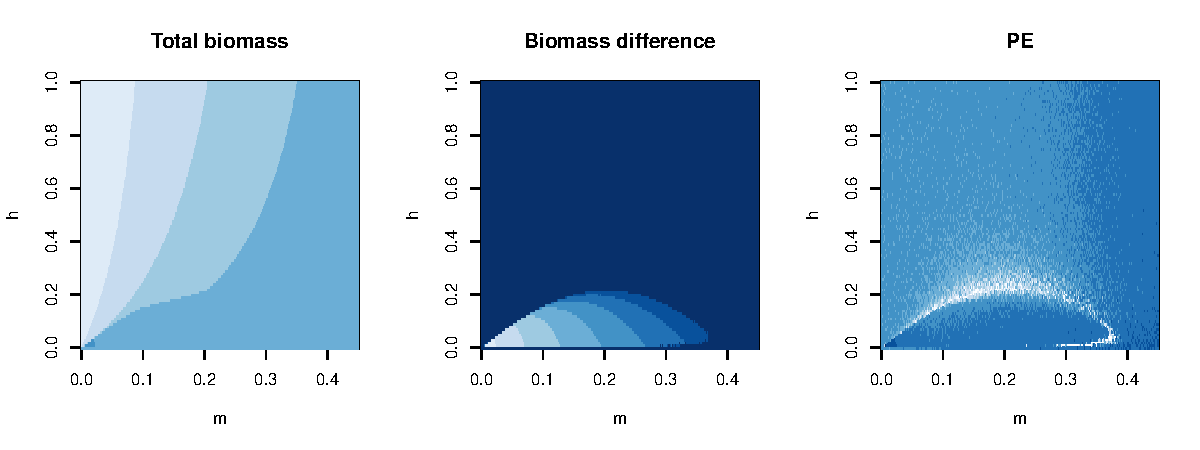
\includegraphics[width=\textwidth]{figs2/fig_MDPE_hm_theta3.pdf} 
% \caption{Low habitat heterogeneity ($\Delta\theta=3$)} \label{fig:thetadiff1}
% \end{subfigure}
% \begin{subfigure}[t]{0.55\textwidth}
% \centering
% 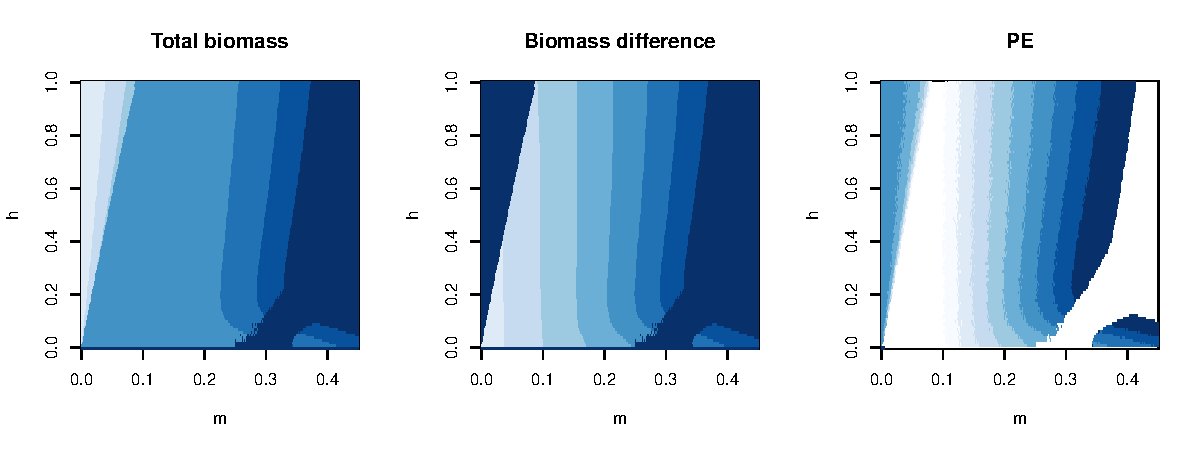
\includegraphics[width=\textwidth]{figs2/fig_MDPE_hm_theta8.pdf} 
% \caption{High habitat heterogeneity ($\Delta\theta=8$)} \label{fig:thetadiff2}
% \end{subfigure}
% \caption{Total means $N_t$, difference in means $\Delta N$, and the portfolio effect PE for different habitat heterogeneities $\Delta\theta$. Light colors = high values.
% }
% \end{figure*}


% \begin{figure*}[h!]
%   \captionsetup{justification=raggedright,
% singlelinecheck=false
% }
% \centering
% 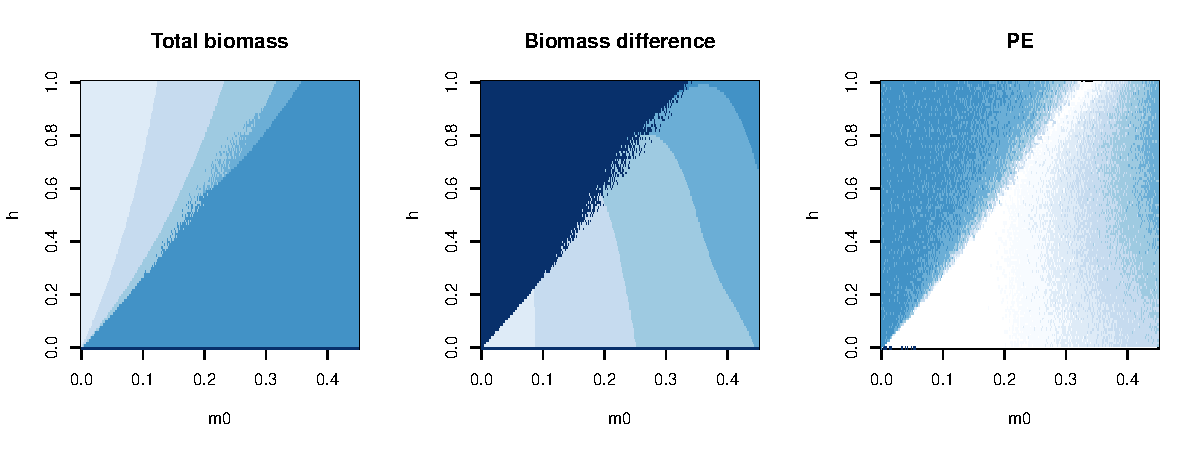
\includegraphics[width=0.8\textwidth]{figs2/fig_MDPE_hm_ddm.pdf}
% \caption{
% The same simulations as presented in Figure \ref{fig:PE}, except with density-dependent straying, where $m(t) = m_0\left(1-N(t)/(C+N(t)\right)$. Light colors = high values.
% } \label{fig:ddm}
% \end{figure*}


\end{document}
